\documentclass[a4paper,12pt]{report}
\usepackage[left=0.75in,right=0.75in,top=1.5in,bottom=1.5in,footskip=.25in]{geometry}
\usepackage[hidelinks]{hyperref}
\usepackage{graphicx}
\usepackage[english]{babel}
\usepackage[utf8]{inputenc}
\usepackage{url}
\usepackage[toc,automake,acronym,section]{glossaries}
\usepackage[section]{placeins} %This package prevents images to shift to other sections.
\usepackage{biblatex}
\addbibresource{ref.bib}
\usepackage[toc,page,header]{appendix}
\usepackage{hhline,colortbl,color,booktabs}
\usepackage{longtable}


\newcommand{\TermName}{FALL 2019}
\newcommand{\Course}{\textbf{SOEN-6481 \vspace{0.5cm} SOFTWARE SYSTEMS REQUIREMENTS SPECIFICATION}}
\newcommand{\ProfessorName}{Dr. PANKAJ KAMTHAN}
\setcounter{chapter}{1}



%---------------------------------------------------------------------------------------
%  GLOSSORY
%---------------------------------------------------------------------------------------

\newglossaryentry{US}
{
	name=User Story,
	description={User Story}
}
\newglossaryentry{tvm}
{
	name=Ticket Vending Machine,
	description={Ticket Vending Machine}
}
\newglossaryentry{iGO}
{
	name=iGO,
	description={Name of the TVM}
}
\newglossaryentry{Administrator}
{
	name=Administrator,
	description={Electronic Method of Payment}
}
\newglossaryentry{Commuter}
{
	name=Quality Commuter,
	description={Someone who is using the transport service to travel}
}
\newglossaryentry{Rational_User}
{
	name=Rational User,
	description={A practical User}
}
\newglossaryentry{Idealist_User}
{
	name=Idealist User,
	description={person guided by principles or hopes rather than by practicality.}
}
\newglossaryentry{competitor}
{
	name=Competitors,
	description={Type of negative stakeholders, this category consist of an organisation or an individual that can be compitition for the developers of iGo}
}
\newglossaryentry{modular_system_design}
{
	name=Modular,
	description={Is a approach that subdivides a system into smaller parts called modules}
}
\newglossaryentry{security_vulnerability}
{
	name=Security Vulnerability,
	description={In computer security, a vulnerability is a weakness which can be exploited by a threat actor, such as an attacker, to perform unauthorized actions within a computer system.}
}
\newglossaryentry{concession}
{
	name=Concession,
	description={A preferential allowance on the ticket.}
}
\newglossaryentry{TMIGO}
{
	name=TMIGO,
	description={Traceability Matrix for iGO.}
}
\newglossaryentry{rechargable_card}
{
	name=Rechargable Card,
	description={A card that can be recharged to be used monthly, weekly.}
}
\newglossaryentry{non_rechargable_card}
{
	name=Non-Rechargable Card,
	description={One time use and throw card.}
}

\newacronym{stm}{STM}{Société de transport de Montréal}

\makeglossary

\begin{document}

%----------------------------------------------------------------------------------------
%	TITLE PAGE START
%----------------------------------------------------------------------------------------

\begin{titlepage}
\newcommand{\HRule}{\rule{\linewidth}{0.5mm}} %New command for thickness of line	


\centering
\textbf{\LARGE  Concordia University} \\ [5mm] 

\includegraphics[scale=.1]{University_logo.jpg}\\[1cm] 
\textsc{\Large \Course (\TermName)} \\  [0.5cm]

%--------
%	TITLE
%--------
	
\HRule \\[0.4cm]
{ \huge \bfseries TICKET VENDING MACHINE}\\[0.4cm] 
\HRule \\[0.5cm]

{\large \textbf{DELIVERABLE 2 (D2)} }	

\HRule \\[1.5cm]
%---------
%	TAIL SECTION OF TITLE PAGE
%---------
\vspace{3cm}

\begin{flushleft}


\textbf{\underline{\Large Submitted By: (Team E)}}
\hfill
\textbf{\underline{\Large Submitted To:}} \\
\vspace{3mm}
\large Bhavpreet Kaur (40071697)
\hfill
\large Prof. Pankaj Kamthan \\

\large Navjot Kaur (40078155) \hfill \\
\large Mehrnaz Keshmirpour (40063320) \hfill \\
\large Shruthi Kondapura Venkataiah (40091427) \hfill \\
\large Sanchit Kumar (40081187	) \\

\end{flushleft}

\centering \vspace{1cm}

GitHub - \href{https://github.com/m3hrn4z/SRS}{https://github.com/m3hrn4z/SRS}

\vspace{0.1cm}
{\large \today}\\[2cm]

\vfill
\end{titlepage}


%---------
%	TABLE OF CONTENT PAGE
%---------

\newpage

\tableofcontents



%---------
%	NEW PAGE
%---------

\chapter*{\centering Deliverable - 2}

\vspace{1cm}
\section{Problem 5: Personas \cite{usermodelingkamthan}}

\FloatBarrier
\subsection{Student}
\begin{figure}[!htb]
	\fbox{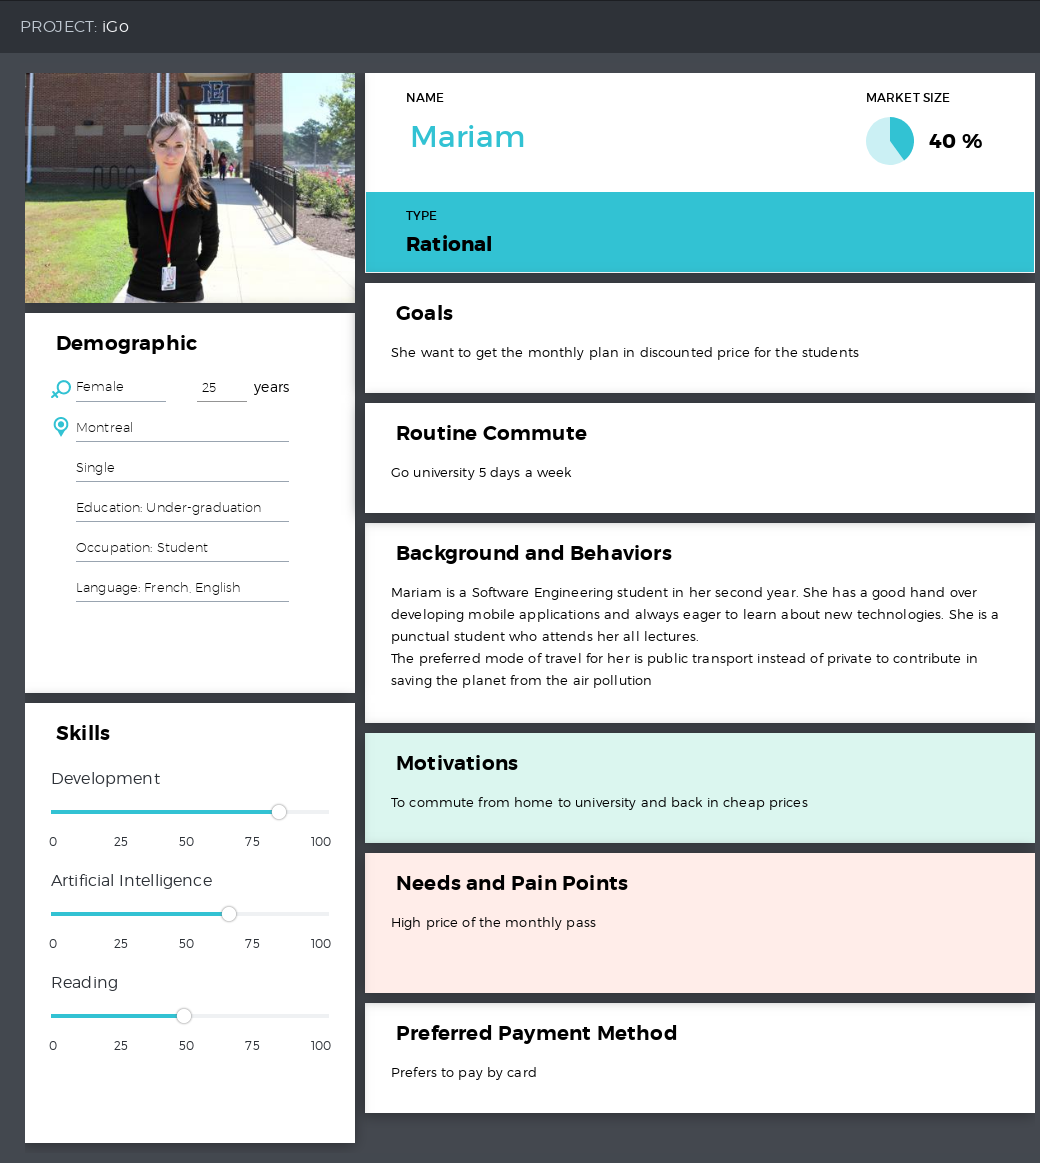
\includegraphics[width=18cm, height=20cm]{Personas/Student.png}}
	\caption{\label{fig:persona_student}Persona: Student}	
\end{figure}

\FloatBarrier
\subsection{Professional}
\begin{figure}[!htb]
	\fbox{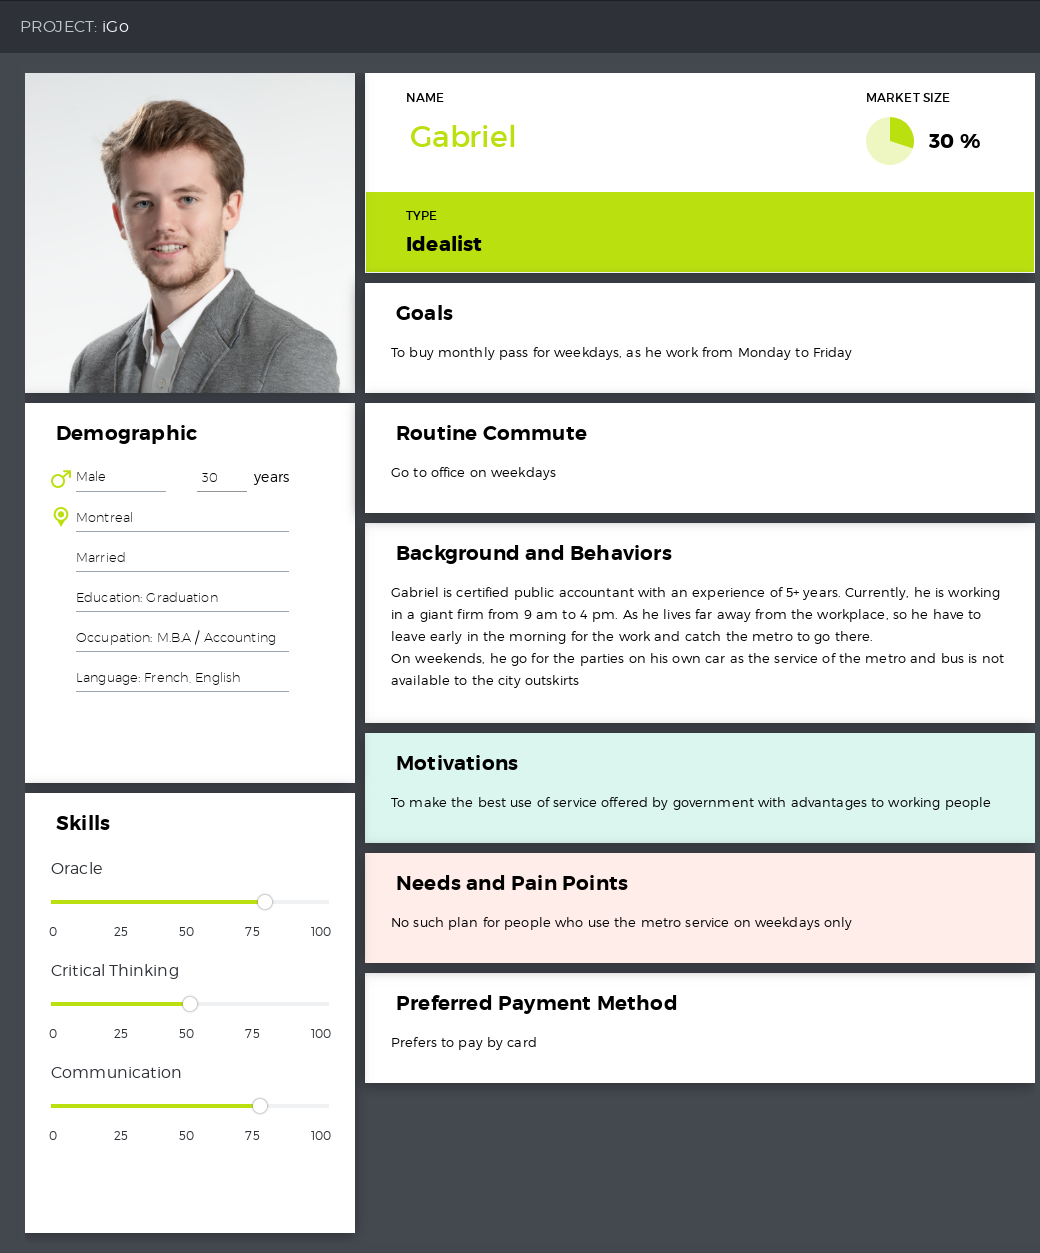
\includegraphics[width=18cm, height=19cm]{Personas/WorkingProfessional.png}}
	\caption{\label{fig:working_professional}Persona: Working Professional}	
\end{figure}

\FloatBarrier
\subsection{Senior Citizen}
\begin{figure}[!htb]
	\fbox{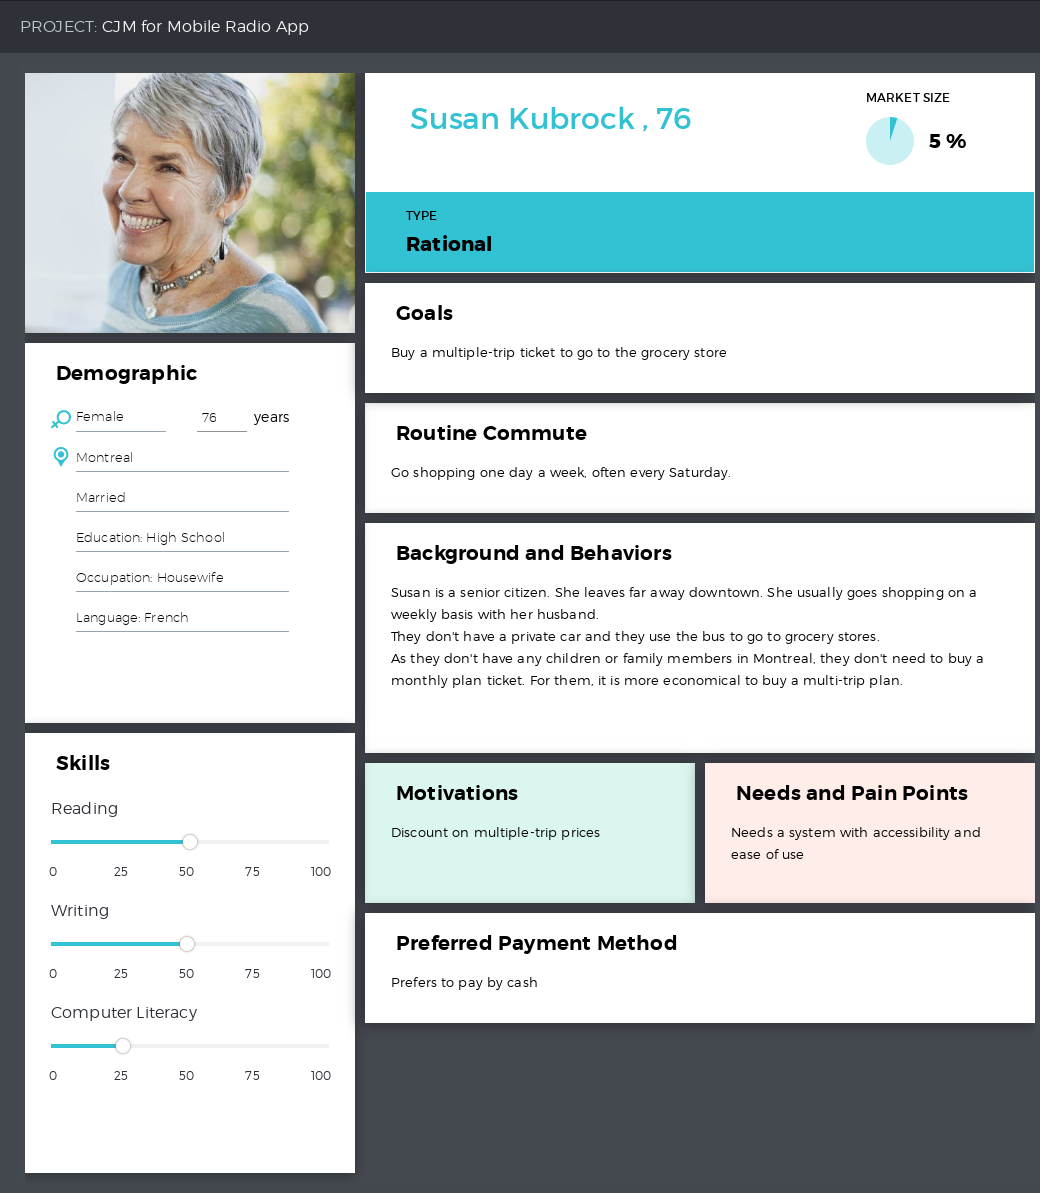
\includegraphics[width=18cm, height=19cm]{Personas/SeniorCitizen.png}}
	\caption{\label{fig:senior_citizen}Persona: Senior Citizen}	
\end{figure}

\FloatBarrier
\subsection{Occasional traveller}
\begin{figure}[!htb]
	\fbox{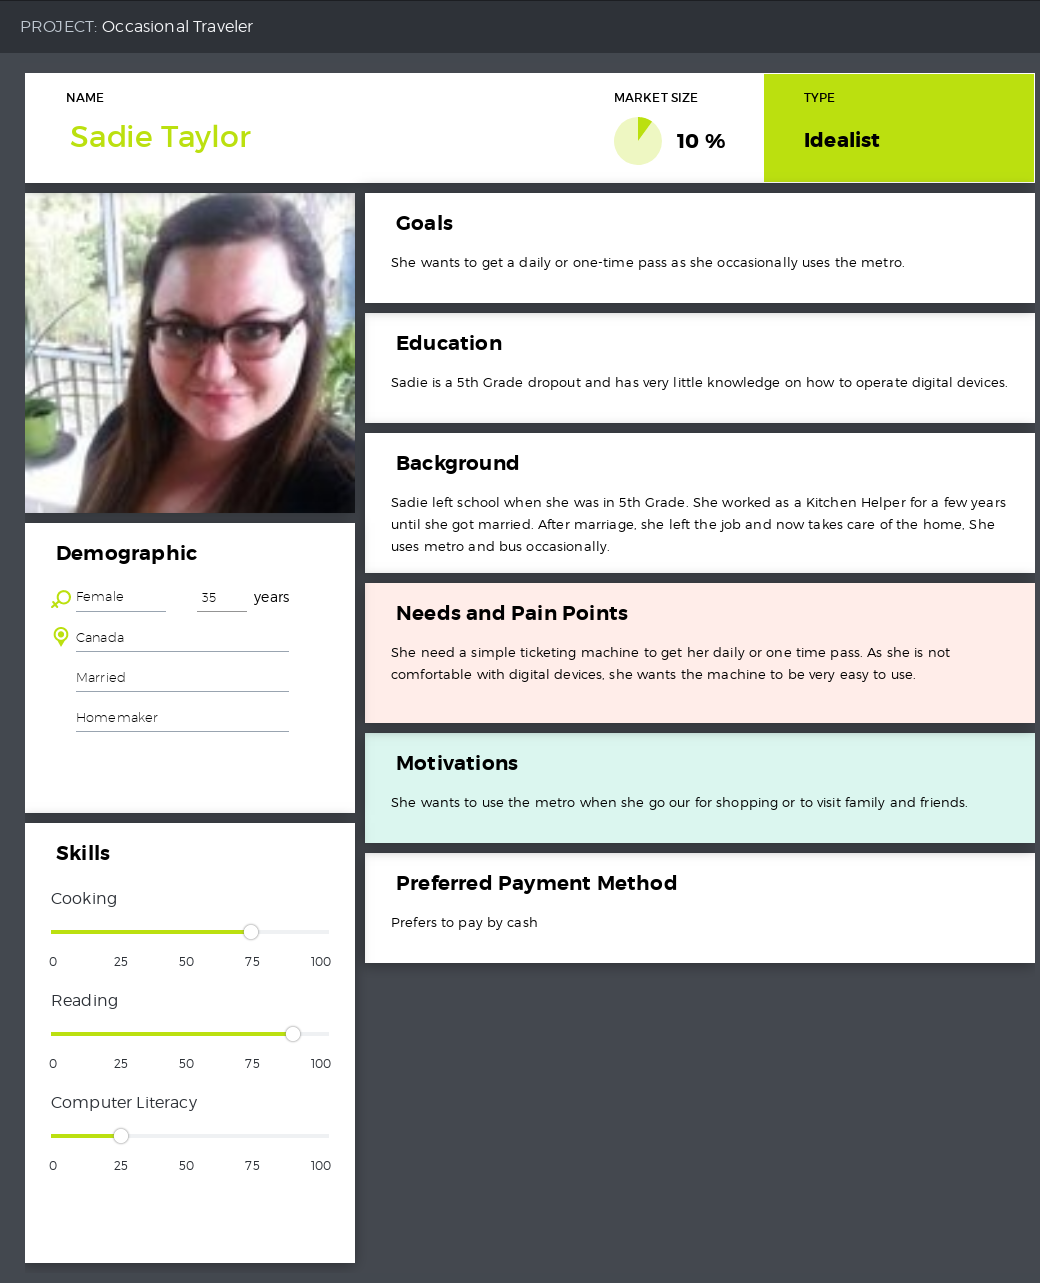
\includegraphics[width=18cm, height=19cm]{Personas/OccasionalTraveller.png}}
	\caption{\label{fig:occasional_traveller}Persona: Occasional Traveller}	
\end{figure}

\FloatBarrier
\subsection{Frequent Traveller}
\begin{figure}[!htb]
	\fbox{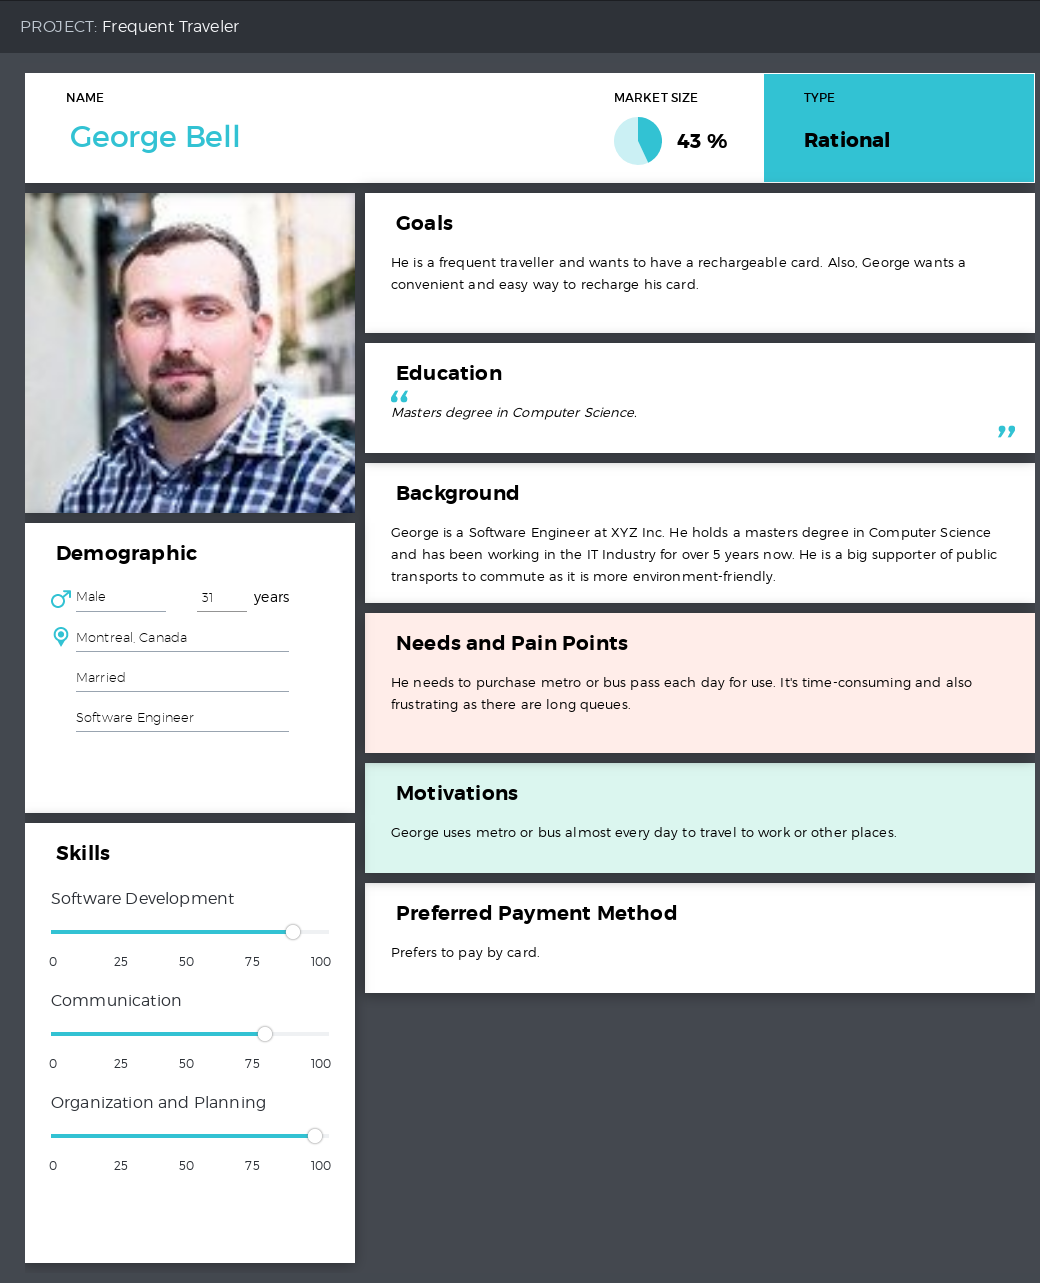
\includegraphics[width=18cm, height=19cm]{Personas/FrequentTraveller.png}}
	\caption{\label{fig:frequent_traveller}Persona: Frequent Traveller}	
\end{figure}

\FloatBarrier
\subsection{Visually Impaired}
\begin{figure}[!htb]
	\fbox{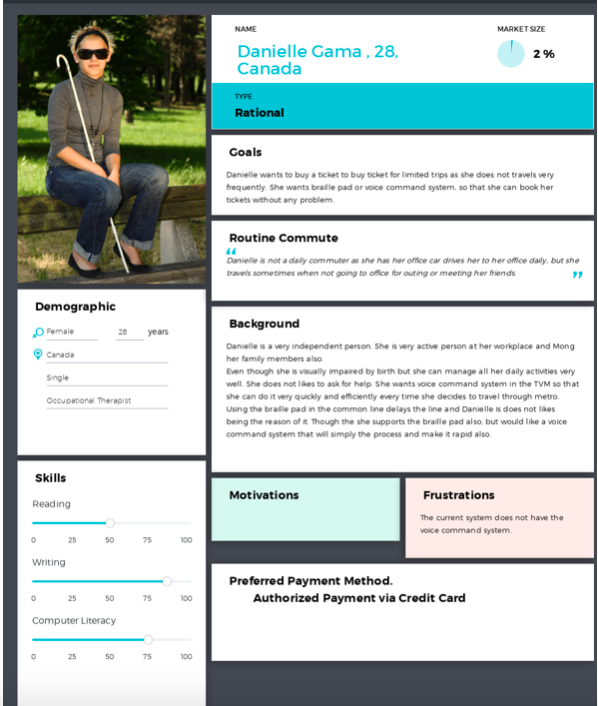
\includegraphics[width=18cm, height=19cm]{Personas/VisuallyImpaired.png}}
	\caption{\label{fig:visually_impaired}Persona: Visually Impaired}	
\end{figure}

\FloatBarrier
\subsection{Differently Abled}
\begin{figure}[!htb]
	\fbox{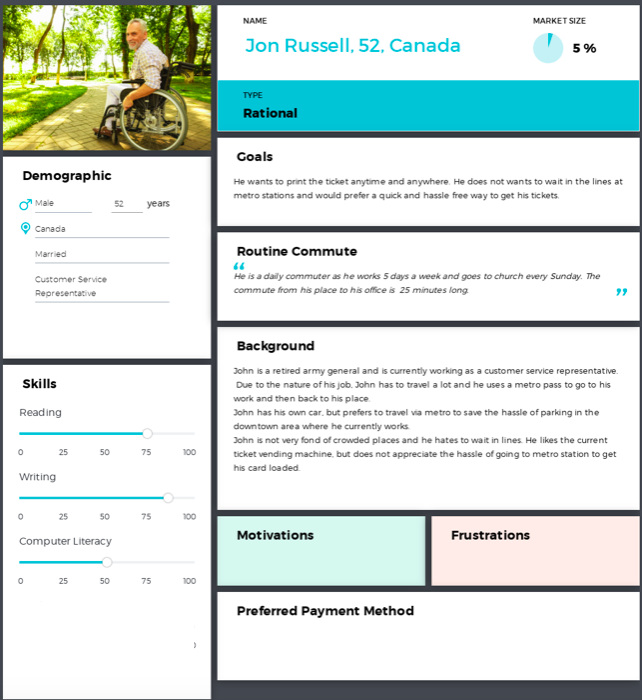
\includegraphics[width=18cm, height=19cm]{Personas/DifferentlyAbled.png}}
	\caption{\label{fig:differently_abled}Persona: Differently Abled}	
\end{figure}

\FloatBarrier
\subsection{Negative User}
\begin{figure}[!htb]
	\fbox{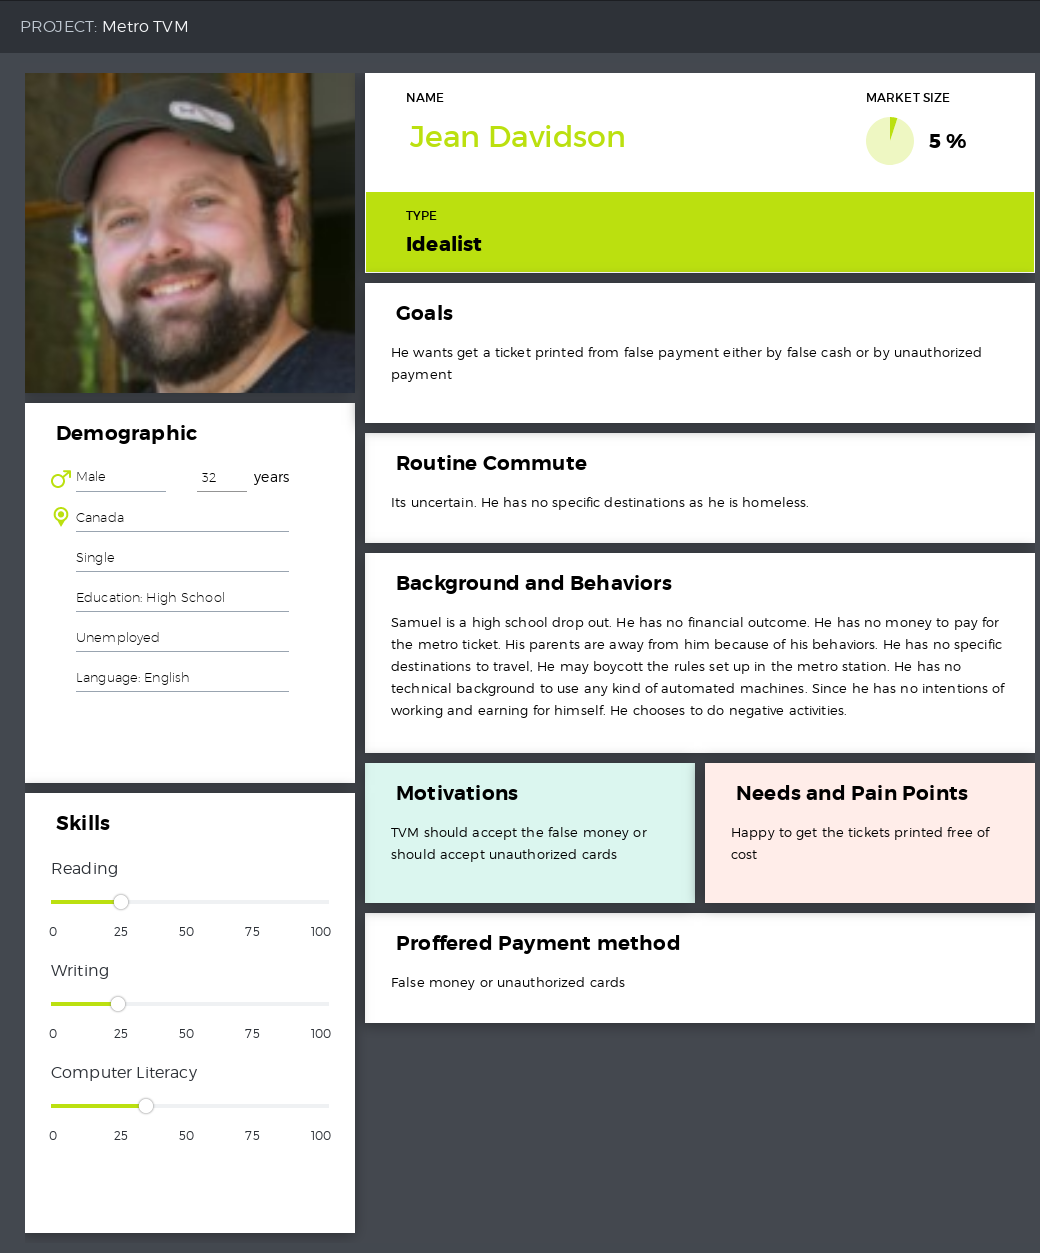
\includegraphics[width=18cm, height=19cm]{Personas/NegativePersona1.png}}
	\caption{\label{fig:negative_persona_1}Persona: Negative Persona 1}	
\end{figure}

\FloatBarrier
\subsection{Negative User: Hacker}
\begin{figure}[!htb]
	\fbox{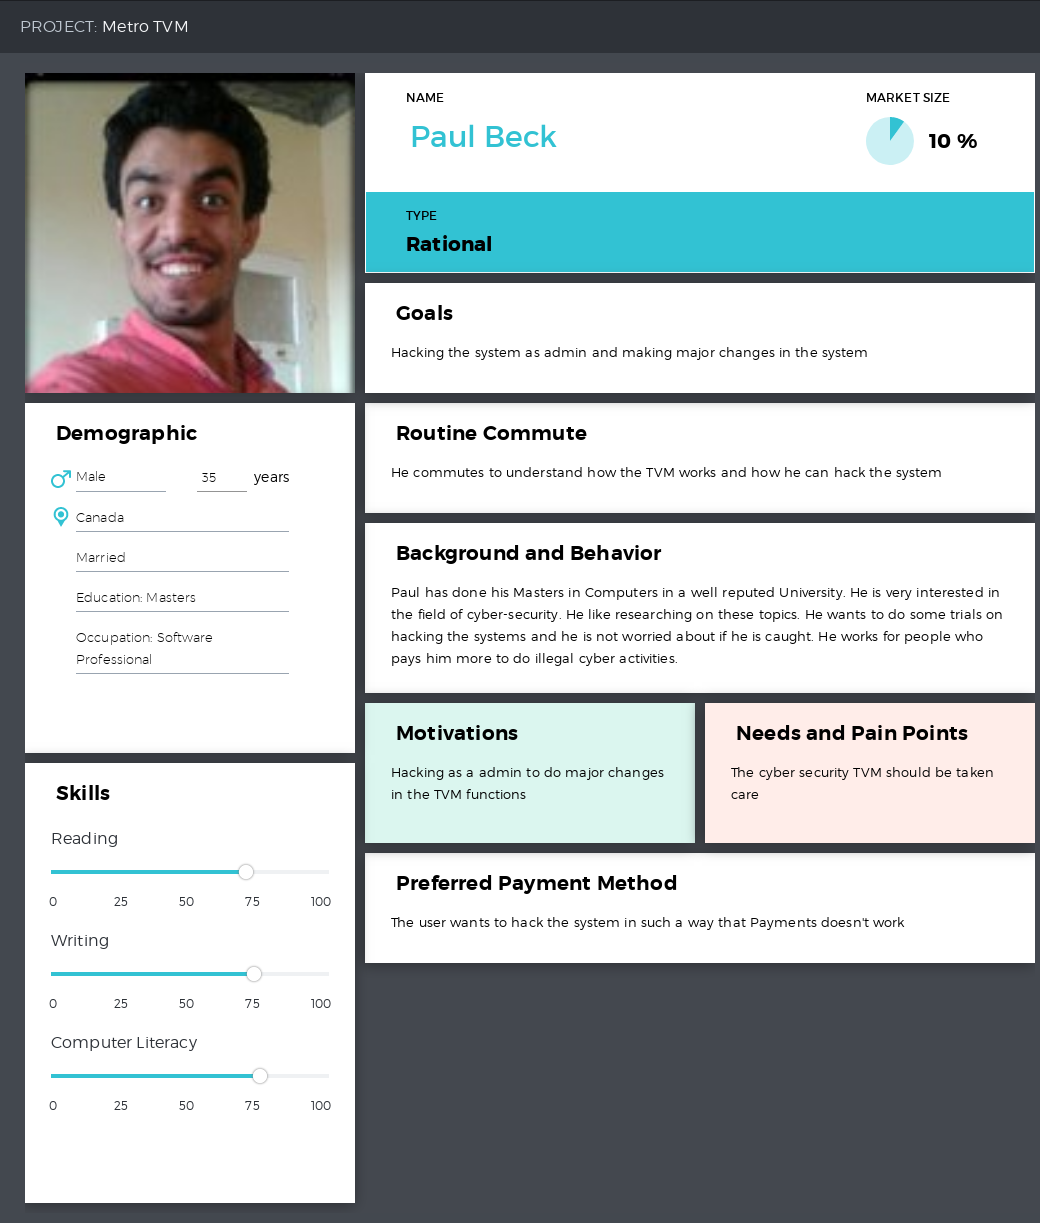
\includegraphics[width=18cm, height=19cm]{Personas/NegativePersona2.png}}
	\caption{\label{fig:negative_persona_hacker}Persona: Negative Persona: Hacker}	
\end{figure}




\section{Problem 5: Global Constraints}

\begin{longtable}{ | p{0.2\linewidth} | p{0.6\linewidth} | }
	\hline
	
	 & \\ %Blank line
	\centering \textbf{ID}  & \textbf{Constraint} \\
	& \\ %Blank line
	\hline
	
	
	& \\ %Blank line
	Performance-G-01 & From the time user selects to interact with the system, it takes less than or equal to 5 seconds on average for the system to display the result to that user. \\
	& \\ %Blank line
	\hline
	
	& \\ %Blank line
	Usability-G-01 & User is able to go back to previous step and modify the request. \\
		& \\ %Blank line
	\hline
	
	& \\ %Blank line
	Accessibility-G-01 & \gls{tvm} is accessible by users with different backgrounds and abilities by using a screen reader for vision impaired users or people who cannot read/write. \\
	& \\ %Blank line
	\hline
	
	& \\ %Blank line
	Maintainability-G-01: & Admin can modify system parameters and make changes later, without effecting current functionality of the system \\
	& \\ %Blank line
	\hline
	
	& \\ %Blank line
	Security-G-01 & The server on which the system resides has its own security to prevent unauthorized read and wirte and delete access. \\
	& \\ %Blank line
	\hline
	
	& \\ %Blank line
	Privacy-G-01 & The information regarding bank card is not saved on the server. \\
	& \\ %Blank line
	\hline
	
	& \\ %Blank line
	Privacy-G-02 & Personal information of registered users is accessible only by authorized people. \\
	& \\ %Blank line
	\hline

\end{longtable}


\vspace{1cm}
\section{Problem 5: User Stories \cite{userstorieskamthan}}


\textbf{Quality of User Stories \cite{qualitykamthan}} \\

\textbf{Systematic scheme:} We have a framework for user stories within the team to describe the user stories. The user story framework gives details about the constraints to be followed, list of acceptance tests and also the inspired user roles and personas.\\


\textbf{Characteristics of user stories considered:} \\ 
\textbf{I-Investable —} User stories are written in such a way that a team should be able to invest their time and resources. \\
\textbf{N-Negotiable —} Team members are able to discuss around its impacts, edge cases and expected behaviour. \\
\textbf{V-Valuable —} User stories are with significant business/ technical value into the product. \\
\textbf{E-Estimable —} User story points are assigned to each user stories based on their effort of development \\
\textbf{S-Small —} user stories are small enough that a scrum team can deliver within a sprint length. \\
\textbf{T-Testable —} written acceptance test cases for each user stories, which means they are testable \\


\textbf{Individually as well as communally:} User stories are independent, we will be are able to implement user stories individually. They are communal, which means they are following the same format of description, they are having the same characteristics but different implementations. They are \gls{modular_system_design} so that they can be integrated and very easy for maintenance.







\setlength\arrayrulewidth{2pt}
\FloatBarrier


%==================================================================================
%				Customer Login
%==================================================================================


\subsection{User Story : Customer Login}

\begin{longtable}{!{\color{blue}\vrule width 5pt} p{0.4\linewidth} | p{0.15\linewidth} | p{0.2\linewidth} !{\color{blue}\vrule width 5pt} }
	
	
	\noalign{\global\arrayrulewidth=1mm}
	\arrayrulecolor{blue}\hline
	\noalign{\global\arrayrulewidth=0.5mm}
	\arrayrulecolor{black}\hline
	%\arrayrulecolor{blue} \linethickness{3}  \hline \arrayrulecolor{black}
	
	
	& & \\
	\textbf{Title: Customer Login} & \textbf{Priority: } & \textbf{Estimate:} \\
	& & \\
	\textbf{ID: TVM-01	} & High & 3 (story points) \\
	& & \\
	\hline	
	
	%User story statement
	\multicolumn{3}{!{\color{blue}\vrule width 5pt} p{0.9\linewidth} !{\color{blue}\vrule width 5pt}}{\space} \\ %Blank line
	\multicolumn{3}{!{\color{blue}\vrule width 5pt} l !{\color{blue}\vrule width 5pt}}{\textbf{As a} \gls{Commuter}} \\ 
	\multicolumn{3}{!{\color{blue}\vrule width 5pt} l !{\color{blue}\vrule width 5pt}}{\textbf{I want to} login to the TVM system} \\
	\multicolumn{3}{!{\color{blue}\vrule width 5pt} l !{\color{blue}\vrule width 5pt}}{\textbf{So that I can} view my ticket plans} \\
	\multicolumn{3}{!{\color{blue}\vrule width 5pt} p{0.9\linewidth} !{\color{blue}\vrule width 5pt}}{\space} \\ %Blank line
	\hline
	
	
	%Constraint Section
	\multicolumn{3}{!{\color{blue}\vrule width 5pt} p{0.9\linewidth} !{\color{blue}\vrule width 5pt}}{\space} \\ %Blank line
	
	\multicolumn{3}{!{\color{blue}\vrule width 5pt} p{0.9\linewidth} !{\color{blue}\vrule width 5pt}}{\textbf{Constraints:} } \\ 

	\multicolumn{3}{!{\color{blue}\vrule width 5pt} p{0.9\linewidth} !{\color{blue}\vrule width 5pt}}{\space} \\ %Blank line
	
	\multicolumn{3}{!{\color{blue}\vrule width 5pt} p{0.9\linewidth} !{\color{blue}\vrule width 5pt}}{\textbf{Performance-G-01, Usability-G-01, Accessibility-G-01, Maintainability-G-01, Security-G-01, Privacy-G-01, Privacy-G-02}} \\
	
	\multicolumn{3}{!{\color{blue}\vrule width 5pt} p{0.9\linewidth} !{\color{blue}\vrule width 5pt}}{\space} \\ %Blank line
	
	\multicolumn{3}{!{\color{blue}\vrule width 5pt} p{0.9\linewidth} !{\color{blue}\vrule width 5pt}}{\textbf{Usability-1:} Login credential text boxes should be prominently visible on the screen} \\
	
	\multicolumn{3}{!{\color{blue}\vrule width 5pt} p{0.9\linewidth} !{\color{blue}\vrule width 5pt}}{\space} \\ %Blank line
	
	\hline
	
	%Acceptance Criteria
	\multicolumn{3}{!{\color{blue}\vrule width 5pt} p{0.9\linewidth} !{\color{blue}\vrule width 5pt}}{\space} \\ %Blank line
	
	\multicolumn{3}{!{\color{blue}\vrule width 5pt} p{0.9\linewidth} !{\color{blue}\vrule width 5pt}}{\textbf{Acceptance criteria:} } \\ 
	
	\multicolumn{3}{!{\color{blue}\vrule width 5pt} p{0.9\linewidth} !{\color{blue}\vrule width 5pt}}{\space} \\ %Blank line
	
	\multicolumn{3}{!{\color{blue}\vrule width 5pt} p{0.9\linewidth} !{\color{blue}\vrule width 5pt}}{\textbf{Given} a commuter interacting with TVM to view ticket plans} \\
	
	\multicolumn{3}{!{\color{blue}\vrule width 5pt} p{0.9\linewidth} !{\color{blue}\vrule width 5pt}}{\textbf{When} user select the button to login} \\
	
	\multicolumn{3}{!{\color{blue}\vrule width 5pt} p{0.9\linewidth} !{\color{blue}\vrule width 5pt}}{\textbf{Then } system displays to select a language, and response time is less than 5 seconds} \\
	
	\multicolumn{3}{!{\color{blue}\vrule width 5pt} p{0.9\linewidth} !{\color{blue}\vrule width 5pt}}{\space} \\ %Blank line
	
	\multicolumn{3}{!{\color{blue}\vrule width 5pt} p{0.9\linewidth} !{\color{blue}\vrule width 5pt}}{\textbf{Usability-Test-1:} User should find the fields easily to enter credentials} \\
	
	\multicolumn{3}{!{\color{blue}\vrule width 5pt} p{0.9\linewidth} !{\color{blue}\vrule width 4pt}}{\textbf{Performance-G-01-Test-1:} User interacts with TVM with speed and ease-of-use. Response time should be acceptable (less than 5 seconds). } \\
	
	\multicolumn{3}{!{\color{blue}\vrule width 5pt} p{0.9\linewidth} !{\color{blue}\vrule width 5pt}}{\space} \\ %Blank line
	
	\multicolumn{3}{!{\color{blue}\vrule width 5pt} p{0.9\linewidth} !{\color{blue}\vrule width 4pt}}{\textbf{Accessibility-G-01-Test-1:} A user can hear the voice asking for TVM login } \\
	
	\multicolumn{3}{!{\color{blue}\vrule width 5pt} p{0.9\linewidth} !{\color{blue}\vrule width 5pt}}{\space} \\ %Blank line
	
	\hline
	
	
	%Relevant Persona
	\multicolumn{3}{!{\color{blue}\vrule width 5pt} p{0.9\linewidth} !{\color{blue}\vrule width 5pt}}{\space} \\ %Blank line
	
	\multicolumn{3}{!{\color{blue}\vrule width 5pt} p{0.9\linewidth} !{\color{blue}\vrule width 5pt}}{\textbf{Relevant Persona(s) / User(s):}} \\
	
	\multicolumn{3}{!{\color{blue}\vrule width 5pt} p{0.9\linewidth} !{\color{blue}\vrule width 5pt}}{Unregistered Commuter, Registered Commuter includes: Regular User, Student, Senior Citizen, Negative user} \\
	
	\multicolumn{3}{!{\color{blue}\vrule width 5pt} p{0.9\linewidth} !{\color{blue}\vrule width 5pt}}{\space} \\ %Blank line
	
	\multicolumn{3}{!{\color{blue}\vrule width 5pt} p{0.9\linewidth} !{\color{blue}\vrule width 5pt}}{\textbf{Personas: }George Bell, Susan Kubrock, Sadie Taylor, Jean Davidson} \\
	
	\multicolumn{3}{!{\color{blue}\vrule width 5pt} p{0.9\linewidth} !{\color{blue}\vrule width 5pt}}{\space} \\ %Blank line
	
	\hline
	
	
	\noalign{\global\arrayrulewidth=1mm}
	\arrayrulecolor{blue}\hline
	\noalign{\global\arrayrulewidth=0.5mm}
	\arrayrulecolor{black}\hline	
	
\end{longtable}



%==================================================================================
%				Select Language
%==================================================================================

\vspace{1cm}
\subsection{User Story : Select Language}

\begin{longtable}{!{\color{blue}\vrule width 5pt} p{0.4\linewidth} | p{0.15\linewidth} | p{0.2\linewidth} !{\color{blue}\vrule width 5pt} }
	
	
	\noalign{\global\arrayrulewidth=1mm}
	\arrayrulecolor{blue}\hline
	\noalign{\global\arrayrulewidth=0.5mm}
	\arrayrulecolor{black}\hline
	%\arrayrulecolor{blue} \linethickness{3}  \hline \arrayrulecolor{black}
	
	
	& & \\
	\textbf{Title: Select Language} & \textbf{Priority: } & \textbf{Estimate:} \\
	& & \\
	\textbf{ID: TVM-02	} & Medium & 2 (story points) \\
	& & \\
	\hline	
	
	%User story statement
	\multicolumn{3}{!{\color{blue}\vrule width 5pt} p{0.9\linewidth} !{\color{blue}\vrule width 5pt}}{\space} \\ %Blank line
	\multicolumn{3}{!{\color{blue}\vrule width 5pt} l !{\color{blue}\vrule width 5pt}}{\textbf{As a} commuter} \\ 
	\multicolumn{3}{!{\color{blue}\vrule width 5pt} l !{\color{blue}\vrule width 5pt}}{\textbf{I want to} select language} \\
	\multicolumn{3}{!{\color{blue}\vrule width 5pt} l !{\color{blue}\vrule width 5pt}}{\textbf{So that I can} interact with TVM system} \\
	\multicolumn{3}{!{\color{blue}\vrule width 5pt} p{0.9\linewidth} !{\color{blue}\vrule width 5pt}}{\space} \\ %Blank line
	\hline
	
	
	%Constraint Section
	\multicolumn{3}{!{\color{blue}\vrule width 5pt} p{0.9\linewidth} !{\color{blue}\vrule width 5pt}}{\space} \\ %Blank line
	
	\multicolumn{3}{!{\color{blue}\vrule width 5pt} p{0.9\linewidth} !{\color{blue}\vrule width 5pt}}{\textbf{Constraints:} } \\ 
	
	\multicolumn{3}{!{\color{blue}\vrule width 5pt} p{0.9\linewidth} !{\color{blue}\vrule width 5pt}}{\space} \\ %Blank line
	
	\multicolumn{3}{!{\color{blue}\vrule width 5pt} p{0.9\linewidth} !{\color{blue}\vrule width 5pt}}{\textbf{Performance-G-01, Accessibility-G-01, Maintainability-G-01}} \\
	
	\multicolumn{3}{!{\color{blue}\vrule width 5pt} p{0.9\linewidth} !{\color{blue}\vrule width 5pt}}{\space} \\ %Blank line
	
	\multicolumn{3}{!{\color{blue}\vrule width 5pt} p{0.9\linewidth} !{\color{blue}\vrule width 5pt}}{\textbf{Usability-1:} User should be given list of language options to choose} \\
	
	\multicolumn{3}{!{\color{blue}\vrule width 5pt} p{0.9\linewidth} !{\color{blue}\vrule width 5pt}}{\space} \\ %Blank line
	
	\hline
	
	%Acceptance Criteria
	\multicolumn{3}{!{\color{blue}\vrule width 5pt} p{0.9\linewidth} !{\color{blue}\vrule width 5pt}}{\space} \\ %Blank line
	
	\multicolumn{3}{!{\color{blue}\vrule width 5pt} p{0.9\linewidth} !{\color{blue}\vrule width 5pt}}{\textbf{Acceptance criteria:} } \\ 
	
	\multicolumn{3}{!{\color{blue}\vrule width 5pt} p{0.9\linewidth} !{\color{blue}\vrule width 5pt}}{\space} \\ %Blank line
	
	\multicolumn{3}{!{\color{blue}\vrule width 5pt} p{0.9\linewidth} !{\color{blue}\vrule width 5pt}}{\textbf{Given} a commuter interacting with TVM to select known language} \\
	
	\multicolumn{3}{!{\color{blue}\vrule width 5pt} p{0.9\linewidth} !{\color{blue}\vrule width 5pt}}{\textbf{When} selects the known language} \\
	
	\multicolumn{3}{!{\color{blue}\vrule width 5pt} p{0.9\linewidth} !{\color{blue}\vrule width 5pt}}{\textbf{Then } system displays the next information in selected language, and response time is less than 5 seconds} \\
	
	\multicolumn{3}{!{\color{blue}\vrule width 5pt} p{0.9\linewidth} !{\color{blue}\vrule width 5pt}}{\space} \\ %Blank line
	
	\multicolumn{3}{!{\color{blue}\vrule width 5pt} p{0.9\linewidth} !{\color{blue}\vrule width 5pt}}{\textbf{Usability-1-Test-1:} User should be able to easily select the option in the list} \\
	
	\multicolumn{3}{!{\color{blue}\vrule width 5pt} p{0.9\linewidth} !{\color{blue}\vrule width 4pt}}{\textbf{Performance-G-01-Test-1:} User interacts with TVM with speed and ease-of-use. Response time should be acceptable (less than 5 seconds).} \\
	
	\multicolumn{3}{!{\color{blue}\vrule width 5pt} p{0.9\linewidth} !{\color{blue}\vrule width 5pt}}{\space} \\ %Blank line
	
	\multicolumn{3}{!{\color{blue}\vrule width 5pt} p{0.9\linewidth} !{\color{blue}\vrule width 5pt}}{\textbf{Accessibility-G-01-Test-1: }A user can hear the voice asking for language selection} \\
	
	\multicolumn{3}{!{\color{blue}\vrule width 5pt} p{0.9\linewidth} !{\color{blue}\vrule width 5pt}}{\space} \\ %Blank line

	\multicolumn{3}{!{\color{blue}\vrule width 5pt} p{0.9\linewidth} !{\color{blue}\vrule width 5pt}}{\textbf{Maintainability-G-01-Test-1: } A user should get the newly added language options to choose} \\ 
	
	\multicolumn{3}{!{\color{blue}\vrule width 5pt} p{0.9\linewidth} !{\color{blue}\vrule width 5pt}}{\space} \\ %Blank line
	
	\hline
	
	
	%Relevant Persona
	\multicolumn{3}{!{\color{blue}\vrule width 5pt} p{0.9\linewidth} !{\color{blue}\vrule width 5pt}}{\space} \\ %Blank line
	
	\multicolumn{3}{!{\color{blue}\vrule width 5pt} p{0.9\linewidth} !{\color{blue}\vrule width 5pt}}{\textbf{Relevant Persona(s) / User(s):}} \\
	
	\multicolumn{3}{!{\color{blue}\vrule width 5pt} p{0.9\linewidth} !{\color{blue}\vrule width 5pt}}{Unregistered Commuter, Registered Commuter includes: Regular User, Student, Senior Citizen} \\
	
	\multicolumn{3}{!{\color{blue}\vrule width 5pt} p{0.9\linewidth} !{\color{blue}\vrule width 5pt}}{\space} \\ %Blank line
	
	\multicolumn{3}{!{\color{blue}\vrule width 5pt} p{0.9\linewidth} !{\color{blue}\vrule width 5pt}}{\textbf{Personas: }George Bell, Susan Kubrock, Sadie Taylor} \\
	
	\multicolumn{3}{!{\color{blue}\vrule width 5pt} p{0.9\linewidth} !{\color{blue}\vrule width 5pt}}{\space} \\ %Blank line
	
	\hline
	
	
	\noalign{\global\arrayrulewidth=1mm}
	\arrayrulecolor{blue}\hline
	\noalign{\global\arrayrulewidth=0.5mm}
	\arrayrulecolor{black}\hline	
	
\end{longtable}




%==================================================================================
%				Select Ticket Type
%==================================================================================

\vspace{1cm}
\subsection{User Story : Select Ticket Type}

\begin{longtable}{!{\color{blue}\vrule width 5pt} p{0.4\linewidth} | p{0.15\linewidth} | p{0.2\linewidth} !{\color{blue}\vrule width 5pt} }
	
	
	\noalign{\global\arrayrulewidth=1mm}
	\arrayrulecolor{blue}\hline
	\noalign{\global\arrayrulewidth=0.5mm}
	\arrayrulecolor{black}\hline
	%\arrayrulecolor{blue} \linethickness{3}  \hline \arrayrulecolor{black}
	
	
	& & \\
	\textbf{Title: Select Ticket Type} & \textbf{Priority: } & \textbf{Estimate:} \\
	& & \\
	\textbf{ID: TVM-03	} & High & 3 (story points) \\
	& & \\
	\hline	
	
	%User story statement
	\multicolumn{3}{!{\color{blue}\vrule width 5pt} p{0.9\linewidth} !{\color{blue}\vrule width 5pt}}{\space} \\ %Blank line
	\multicolumn{3}{!{\color{blue}\vrule width 5pt} l !{\color{blue}\vrule width 5pt}}{\textbf{As a} commuter} \\ 
	\multicolumn{3}{!{\color{blue}\vrule width 5pt} l !{\color{blue}\vrule width 5pt}}{\textbf{I want to} select ticket types (Rechargeable card or Non-rechargeable ticket)} \\
	\multicolumn{3}{!{\color{blue}\vrule width 5pt} l !{\color{blue}\vrule width 5pt}}{\textbf{So that I can} either reload Non-rechargeable card or buy a Rechargeable ticket} \\
	\multicolumn{3}{!{\color{blue}\vrule width 5pt} p{0.9\linewidth} !{\color{blue}\vrule width 5pt}}{\space} \\ %Blank line
	\hline
	
	
	%Constraint Section
	\multicolumn{3}{!{\color{blue}\vrule width 5pt} p{0.9\linewidth} !{\color{blue}\vrule width 5pt}}{\space} \\ %Blank line
	
	\multicolumn{3}{!{\color{blue}\vrule width 5pt} p{0.9\linewidth} !{\color{blue}\vrule width 5pt}}{\textbf{Constraints:} } \\ 
	
	\multicolumn{3}{!{\color{blue}\vrule width 5pt} p{0.9\linewidth} !{\color{blue}\vrule width 5pt}}{\space} \\ %Blank line
	
	\multicolumn{3}{!{\color{blue}\vrule width 5pt} p{0.9\linewidth} !{\color{blue}\vrule width 5pt}}{\textbf{Performance-G-01, Accessibility-G-01, Maintainability-G-01}} \\
	
	\multicolumn{3}{!{\color{blue}\vrule width 5pt} p{0.9\linewidth} !{\color{blue}\vrule width 5pt}}{\space} \\ %Blank line
	
	\multicolumn{3}{!{\color{blue}\vrule width 5pt} p{0.9\linewidth} !{\color{blue}\vrule width 5pt}}{\textbf{Usability-1:} All ticket types should be displayed on the screen at the same time} \\
	
	\multicolumn{3}{!{\color{blue}\vrule width 5pt} p{0.9\linewidth} !{\color{blue}\vrule width 5pt}}{\space} \\ %Blank line
	
	\hline
	
	%Acceptance Criteria
	\multicolumn{3}{!{\color{blue}\vrule width 5pt} p{0.9\linewidth} !{\color{blue}\vrule width 5pt}}{\space} \\ %Blank line
	
	\multicolumn{3}{!{\color{blue}\vrule width 5pt} p{0.9\linewidth} !{\color{blue}\vrule width 5pt}}{\textbf{Acceptance criteria:} } \\ 
	
	\multicolumn{3}{!{\color{blue}\vrule width 5pt} p{0.9\linewidth} !{\color{blue}\vrule width 5pt}}{\space} \\ %Blank line
	
	\multicolumn{3}{!{\color{blue}\vrule width 5pt} p{0.9\linewidth} !{\color{blue}\vrule width 5pt}}{\textbf{Given} a commuter interacting with TVM to select ticket types} \\
	
	\multicolumn{3}{!{\color{blue}\vrule width 5pt} p{0.9\linewidth} !{\color{blue}\vrule width 5pt}}{\textbf{When} user enter the system to buy a ticket or view ticket plans} \\
	
	\multicolumn{3}{!{\color{blue}\vrule width 5pt} p{0.9\linewidth} !{\color{blue}\vrule width 5pt}}{\textbf{Then } system displays ticket types for user to select among them} \\
	
	\multicolumn{3}{!{\color{blue}\vrule width 5pt} p{0.9\linewidth} !{\color{blue}\vrule width 5pt}}{\space} \\ %Blank line
	
	\multicolumn{3}{!{\color{blue}\vrule width 5pt} p{0.9\linewidth} !{\color{blue}\vrule width 5pt}}{\textbf{Usability-1-Test-1:} A user enters the system and all ticket types will be displayed on the screen for the user to select among them} \\
	
	\multicolumn{3}{!{\color{blue}\vrule width 5pt} p{0.9\linewidth} !{\color{blue}\vrule width 4pt}}{\textbf{Performance-G-01-Test-1:} A user enters the system and the ticket types will be displayed in less than or equal to 5 seconds for the user to select among them} \\
	
	\multicolumn{3}{!{\color{blue}\vrule width 5pt} p{0.9\linewidth} !{\color{blue}\vrule width 5pt}}{\space} \\ %Blank line
	
	\multicolumn{3}{!{\color{blue}\vrule width 5pt} p{0.9\linewidth} !{\color{blue}\vrule width 5pt}}{\textbf{Accessibility-G-01-Test-1: }A user can hear the voice for each text displayed on the output device.} \\
	
	\multicolumn{3}{!{\color{blue}\vrule width 5pt} p{0.9\linewidth} !{\color{blue}\vrule width 5pt}}{\space} \\ %Blank line
	
	\multicolumn{3}{!{\color{blue}\vrule width 5pt} p{0.9\linewidth} !{\color{blue}\vrule width 5pt}}{\textbf{Maintainability-G-01-Test-1: } A system \gls{Administrator} adds a new ticket type without effecting the current functionality of the system} \\ 
	
	\multicolumn{3}{!{\color{blue}\vrule width 5pt} p{0.9\linewidth} !{\color{blue}\vrule width 5pt}}{\space} \\ %Blank line
	
	\hline
	
	
	%Relevant Persona
	\multicolumn{3}{!{\color{blue}\vrule width 5pt} p{0.9\linewidth} !{\color{blue}\vrule width 5pt}}{\space} \\ %Blank line
	
	\multicolumn{3}{!{\color{blue}\vrule width 5pt} p{0.9\linewidth} !{\color{blue}\vrule width 5pt}}{\textbf{Relevant Persona(s) / User(s):}} \\
	
	\multicolumn{3}{!{\color{blue}\vrule width 5pt} p{0.9\linewidth} !{\color{blue}\vrule width 5pt}}{Unregistered Commuter, Registered Commuter includes: Regular User, Student, Senior Citizen} \\
	
	\multicolumn{3}{!{\color{blue}\vrule width 5pt} p{0.9\linewidth} !{\color{blue}\vrule width 5pt}}{\space} \\ %Blank line
	
	\multicolumn{3}{!{\color{blue}\vrule width 5pt} p{0.9\linewidth} !{\color{blue}\vrule width 5pt}}{\textbf{Personas: }Personas: George Bell, Susan Kubrock, Sadie Taylor} \\
	
	\multicolumn{3}{!{\color{blue}\vrule width 5pt} p{0.9\linewidth} !{\color{blue}\vrule width 5pt}}{\space} \\ %Blank line
	
	\hline
	
	
	\noalign{\global\arrayrulewidth=1mm}
	\arrayrulecolor{blue}\hline
	\noalign{\global\arrayrulewidth=0.5mm}
	\arrayrulecolor{black}\hline	
	
\end{longtable}



%==================================================================================
%				View Ticket Plans for Rechargeable card
%==================================================================================



\vspace{2cm}
\subsection{User Story : View Ticket Plans for Rechargeable card}

\begin{longtable}{!{\color{blue}\vrule width 5pt} p{0.4\linewidth} | p{0.15\linewidth} | p{0.2\linewidth} !{\color{blue}\vrule width 5pt} }
	
	
	\noalign{\global\arrayrulewidth=1mm}
	\arrayrulecolor{blue}\hline
	\noalign{\global\arrayrulewidth=0.5mm}
	\arrayrulecolor{black}\hline
	%\arrayrulecolor{blue} \linethickness{3}  \hline \arrayrulecolor{black}
	
	
	& & \\
	\textbf{Title: View Ticket Plans for Rechargeable card} & \textbf{Priority: } & \textbf{Estimate:} \\
	& & \\
	\textbf{ID: TVM-04	} & High & 5 (story points) \\
	& & \\
	\hline	
	
	%User story statement
	\multicolumn{3}{!{\color{blue}\vrule width 5pt} p{0.9\linewidth} !{\color{blue}\vrule width 5pt}}{\space} \\ %Blank line
	\multicolumn{3}{!{\color{blue}\vrule width 5pt} l !{\color{blue}\vrule width 5pt}}{\textbf{As a} commuter} \\ 
	\multicolumn{3}{!{\color{blue}\vrule width 5pt} l !{\color{blue}\vrule width 5pt}}{\textbf{I want to} view ticket plans on selecting rechargeable card with details and fares} \\
	\multicolumn{3}{!{\color{blue}\vrule width 5pt} l !{\color{blue}\vrule width 5pt}}{\textbf{So that I can} decide what plan is suitable for me to buy} \\
	\multicolumn{3}{!{\color{blue}\vrule width 5pt} p{0.9\linewidth} !{\color{blue}\vrule width 5pt}}{\space} \\ %Blank line
	\hline
	
	
	%Constraint Section
	\multicolumn{3}{!{\color{blue}\vrule width 5pt} p{0.9\linewidth} !{\color{blue}\vrule width 5pt}}{\space} \\ %Blank line
	
	\multicolumn{3}{!{\color{blue}\vrule width 5pt} p{0.9\linewidth} !{\color{blue}\vrule width 5pt}}{\textbf{Constraints:} } \\ 
	
	\multicolumn{3}{!{\color{blue}\vrule width 5pt} p{0.9\linewidth} !{\color{blue}\vrule width 5pt}}{\space} \\ %Blank line
	
	\multicolumn{3}{!{\color{blue}\vrule width 5pt} p{0.9\linewidth} !{\color{blue}\vrule width 5pt}}{\textbf{Performance-G-01, Accessibility-G-01, Maintainability-G-01}} \\
	
	\multicolumn{3}{!{\color{blue}\vrule width 5pt} p{0.9\linewidth} !{\color{blue}\vrule width 5pt}}{\space} \\ %Blank line
	
	\multicolumn{3}{!{\color{blue}\vrule width 5pt} p{0.9\linewidth} !{\color{blue}\vrule width 5pt}}{\textbf{Usability-1:} All the plans should be displayed on the screen so that user can compare them together.} \\
	
	\multicolumn{3}{!{\color{blue}\vrule width 5pt} p{0.9\linewidth} !{\color{blue}\vrule width 5pt}}{\textbf{Usability-2:} Information displayed on the screen should be sorted ascending according to fare.} \\
	
	\multicolumn{3}{!{\color{blue}\vrule width 5pt} p{0.9\linewidth} !{\color{blue}\vrule width 5pt}}{\space} \\ %Blank line
	
	\hline
	
	%Acceptance Criteria
	\multicolumn{3}{!{\color{blue}\vrule width 5pt} p{0.9\linewidth} !{\color{blue}\vrule width 5pt}}{\space} \\ %Blank line
	
	\multicolumn{3}{!{\color{blue}\vrule width 5pt} p{0.9\linewidth} !{\color{blue}\vrule width 5pt}}{\textbf{Acceptance criteria:} } \\ 
	
	\multicolumn{3}{!{\color{blue}\vrule width 5pt} p{0.9\linewidth} !{\color{blue}\vrule width 5pt}}{\space} \\ %Blank line
	
	\multicolumn{3}{!{\color{blue}\vrule width 5pt} p{0.9\linewidth} !{\color{blue}\vrule width 5pt}}{\textbf{Given} a commuter interacting with TVM to view ticket plans} \\
	
	\multicolumn{3}{!{\color{blue}\vrule width 5pt} p{0.9\linewidth} !{\color{blue}\vrule width 5pt}}{\textbf{When} user select to display ticket plans} \\
	
	\multicolumn{3}{!{\color{blue}\vrule width 5pt} p{0.9\linewidth} !{\color{blue}\vrule width 5pt}}{\textbf{Then } system will display different plans of ticket along with their details and fares} \\
	
	\multicolumn{3}{!{\color{blue}\vrule width 5pt} p{0.9\linewidth} !{\color{blue}\vrule width 5pt}}{\space} \\ %Blank line
	
	\multicolumn{3}{!{\color{blue}\vrule width 5pt} p{0.9\linewidth} !{\color{blue}\vrule width 5pt}}{\textbf{Usability-1-Test-1:} A user select to view ticket plans and all plans will be displayed on the screen} \\
	
	\multicolumn{3}{!{\color{blue}\vrule width 5pt} p{0.9\linewidth} !{\color{blue}\vrule width 4pt}}{\textbf{Usability-2-Test-1:} A user select to view ticket plans and all plans will be displayed on the screen on ascending order according to ticket fares} \\
	
	\multicolumn{3}{!{\color{blue}\vrule width 5pt} p{0.9\linewidth} !{\color{blue}\vrule width 5pt}}{\space} \\ %Blank line
	
	\multicolumn{3}{!{\color{blue}\vrule width 5pt} p{0.9\linewidth} !{\color{blue}\vrule width 4pt}}{\textbf{Performance-G-01-Test-1:} A user select to view ticket plans and the result will be displayed in less than or equal to 5 seconds} \\
	
	\multicolumn{3}{!{\color{blue}\vrule width 5pt} p{0.9\linewidth} !{\color{blue}\vrule width 5pt}}{\space} \\ %Blank line
	
	\multicolumn{3}{!{\color{blue}\vrule width 5pt} p{0.9\linewidth} !{\color{blue}\vrule width 5pt}}{\textbf{Accessibility-G-01-Test-1: }A user can hear the voice for each text displayed on the output device.} \\
	
	\multicolumn{3}{!{\color{blue}\vrule width 5pt} p{0.9\linewidth} !{\color{blue}\vrule width 5pt}}{\space} \\ %Blank line
	
	\multicolumn{3}{!{\color{blue}\vrule width 5pt} p{0.9\linewidth} !{\color{blue}\vrule width 5pt}}{\textbf{Maintainability-G-01-Test-1: } A system administrator adds a new ticket plan without effecting the current functionality of the system} \\ 
	
	\multicolumn{3}{!{\color{blue}\vrule width 5pt} p{0.9\linewidth} !{\color{blue}\vrule width 5pt}}{\space} \\ %Blank line
	
	\hline
	
	
	%Relevant Persona
	\multicolumn{3}{!{\color{blue}\vrule width 5pt} p{0.9\linewidth} !{\color{blue}\vrule width 5pt}}{\space} \\ %Blank line
	
	\multicolumn{3}{!{\color{blue}\vrule width 5pt} p{0.9\linewidth} !{\color{blue}\vrule width 5pt}}{\textbf{Relevant Persona(s) / User(s):}} \\
	
	\multicolumn{3}{!{\color{blue}\vrule width 5pt} p{0.9\linewidth} !{\color{blue}\vrule width 5pt}}{Registered Commuter includes: Regular User, Student, Senior Citizen} \\
	
	\multicolumn{3}{!{\color{blue}\vrule width 5pt} p{0.9\linewidth} !{\color{blue}\vrule width 5pt}}{\space} \\ %Blank line
	
	\multicolumn{3}{!{\color{blue}\vrule width 5pt} p{0.9\linewidth} !{\color{blue}\vrule width 5pt}}{\textbf{Personas: }Personas: George Bell, Susan Kubrock} \\
	
	\multicolumn{3}{!{\color{blue}\vrule width 5pt} p{0.9\linewidth} !{\color{blue}\vrule width 5pt}}{\space} \\ %Blank line
	
	\hline
	
	
	\noalign{\global\arrayrulewidth=1mm}
	\arrayrulecolor{blue}\hline
	\noalign{\global\arrayrulewidth=0.5mm}
	\arrayrulecolor{black}\hline	
	
\end{longtable}




%==================================================================================
%				View Ticket Plans for Non-Rechargeable card
%==================================================================================


\vspace{1cm}
\subsection{User Story : View Ticket Plans for Non-Rechargeable card}

\begin{longtable}{!{\color{blue}\vrule width 5pt} p{0.4\linewidth} | p{0.15\linewidth} | p{0.2\linewidth} !{\color{blue}\vrule width 5pt} }
	
	
	\noalign{\global\arrayrulewidth=1mm}
	\arrayrulecolor{blue}\hline
	\noalign{\global\arrayrulewidth=0.5mm}
	\arrayrulecolor{black}\hline
	%\arrayrulecolor{blue} \linethickness{3}  \hline \arrayrulecolor{black}
	
	
	& & \\
	\textbf{Title: View Ticket Plans for Non-Rechargeable card} & \textbf{Priority: } & \textbf{Estimate:} \\
	& & \\
	\textbf{ID: TVM-05	} & High & 5 (story points) \\
	& & \\
	\hline	
	
	%User story statement
	\multicolumn{3}{!{\color{blue}\vrule width 5pt} p{0.9\linewidth} !{\color{blue}\vrule width 5pt}}{\space} \\ %Blank line
	\multicolumn{3}{!{\color{blue}\vrule width 5pt} l !{\color{blue}\vrule width 5pt}}{\textbf{As a} commuter} \\ 
	\multicolumn{3}{!{\color{blue}\vrule width 5pt} l !{\color{blue}\vrule width 5pt}}{\textbf{I want to} view ticket plans on selecting non-rechargeable ticket with details and fares} \\
	\multicolumn{3}{!{\color{blue}\vrule width 5pt} l !{\color{blue}\vrule width 5pt}}{\textbf{So that I can} decide what plan is suitable for me to buy} \\
	\multicolumn{3}{!{\color{blue}\vrule width 5pt} p{0.9\linewidth} !{\color{blue}\vrule width 5pt}}{\space} \\ %Blank line
	\hline
	
	
	%Constraint Section
	\multicolumn{3}{!{\color{blue}\vrule width 5pt} p{0.9\linewidth} !{\color{blue}\vrule width 5pt}}{\space} \\ %Blank line
	
	\multicolumn{3}{!{\color{blue}\vrule width 5pt} p{0.9\linewidth} !{\color{blue}\vrule width 5pt}}{\textbf{Constraints:} } \\ 
	
	\multicolumn{3}{!{\color{blue}\vrule width 5pt} p{0.9\linewidth} !{\color{blue}\vrule width 5pt}}{\space} \\ %Blank line
	
	\multicolumn{3}{!{\color{blue}\vrule width 5pt} p{0.9\linewidth} !{\color{blue}\vrule width 5pt}}{\textbf{Performance-G-01, Accessibility-G-01, Maintainability-G-01}} \\
	
	\multicolumn{3}{!{\color{blue}\vrule width 5pt} p{0.9\linewidth} !{\color{blue}\vrule width 5pt}}{\textbf{Usability-1:} All the plans should be displayed on the screen so that user can compare them together.} \\
	
	\multicolumn{3}{!{\color{blue}\vrule width 5pt} p{0.9\linewidth} !{\color{blue}\vrule width 5pt}}{\textbf{Usability-2:} Information displayed on the screen should be sorted ascending according to fare.} \\
	
	\multicolumn{3}{!{\color{blue}\vrule width 5pt} p{0.9\linewidth} !{\color{blue}\vrule width 5pt}}{\space} \\ %Blank line
	
	\hline
	
	%Acceptance Criteria
	\multicolumn{3}{!{\color{blue}\vrule width 5pt} p{0.9\linewidth} !{\color{blue}\vrule width 5pt}}{\space} \\ %Blank line
	
	\multicolumn{3}{!{\color{blue}\vrule width 5pt} p{0.9\linewidth} !{\color{blue}\vrule width 5pt}}{\textbf{Acceptance criteria:} } \\ 
	
	\multicolumn{3}{!{\color{blue}\vrule width 5pt} p{0.9\linewidth} !{\color{blue}\vrule width 5pt}}{\space} \\ %Blank line
	
	\multicolumn{3}{!{\color{blue}\vrule width 5pt} p{0.9\linewidth} !{\color{blue}\vrule width 5pt}}{\textbf{Given} a commuter interacting with TVM to view ticket plans} \\
	
	\multicolumn{3}{!{\color{blue}\vrule width 5pt} p{0.9\linewidth} !{\color{blue}\vrule width 5pt}}{\textbf{When} user select to display ticket plans} \\
	
	\multicolumn{3}{!{\color{blue}\vrule width 5pt} p{0.9\linewidth} !{\color{blue}\vrule width 5pt}}{\textbf{Then } system will display different plans of ticket along with their details and fares} \\
	
	\multicolumn{3}{!{\color{blue}\vrule width 5pt} p{0.9\linewidth} !{\color{blue}\vrule width 5pt}}{\space} \\ %Blank line
	
	\multicolumn{3}{!{\color{blue}\vrule width 5pt} p{0.9\linewidth} !{\color{blue}\vrule width 5pt}}{\textbf{Usability-1-Test-1:} A user select to view ticket plans and all plans will be displayed on the screen} \\
	
	\multicolumn{3}{!{\color{blue}\vrule width 5pt} p{0.9\linewidth} !{\color{blue}\vrule width 4pt}}{\textbf{Usability-2-Test-1:} A user select to view ticket plans and all plans will be displayed on the screen on ascending order according to ticket fares} \\
	
	\multicolumn{3}{!{\color{blue}\vrule width 5pt} p{0.9\linewidth} !{\color{blue}\vrule width 4pt}}{\textbf{Performance-G-02-Test-1:} A user select to view ticket plans and the result will be displayed in less than or equal to 5 seconds} \\
		
	\multicolumn{3}{!{\color{blue}\vrule width 5pt} p{0.9\linewidth} !{\color{blue}\vrule width 5pt}}{\space} \\ %Blank line
	
	\multicolumn{3}{!{\color{blue}\vrule width 5pt} p{0.9\linewidth} !{\color{blue}\vrule width 5pt}}{\textbf{Accessibility-G-01-Test-1: }A user can hear the voice for each text displayed on the output device.} \\
	
	\multicolumn{3}{!{\color{blue}\vrule width 5pt} p{0.9\linewidth} !{\color{blue}\vrule width 5pt}}{\space} \\ %Blank line
	
	\multicolumn{3}{!{\color{blue}\vrule width 5pt} p{0.9\linewidth} !{\color{blue}\vrule width 5pt}}{\textbf{Maintainability-G-01-Test-1: } A system administrator adds a new ticket plan without effecting the current functionality of the system} \\ 
	
	\multicolumn{3}{!{\color{blue}\vrule width 5pt} p{0.9\linewidth} !{\color{blue}\vrule width 5pt}}{\space} \\ %Blank line
	
	\hline
	
	
	%Relevant Persona
	\multicolumn{3}{!{\color{blue}\vrule width 5pt} p{0.9\linewidth} !{\color{blue}\vrule width 5pt}}{\space} \\ %Blank line
	
	\multicolumn{3}{!{\color{blue}\vrule width 5pt} p{0.9\linewidth} !{\color{blue}\vrule width 5pt}}{\textbf{Relevant Persona(s) / User(s):}} \\
	
	\multicolumn{3}{!{\color{blue}\vrule width 5pt} p{0.9\linewidth} !{\color{blue}\vrule width 5pt}}{Registered Commuter includes: Regular User, Student, Senior Citizen} \\
	
	\multicolumn{3}{!{\color{blue}\vrule width 5pt} p{0.9\linewidth} !{\color{blue}\vrule width 5pt}}{\space} \\ %Blank line
	
	\multicolumn{3}{!{\color{blue}\vrule width 5pt} p{0.9\linewidth} !{\color{blue}\vrule width 5pt}}{\textbf{Personas: }Personas: George Bell, Susan Kubrock, Gabriel, Mariam} \\
	
	\multicolumn{3}{!{\color{blue}\vrule width 5pt} p{0.9\linewidth} !{\color{blue}\vrule width 5pt}}{\space} \\ %Blank line
	
	\hline
	
	
	\noalign{\global\arrayrulewidth=1mm}
	\arrayrulecolor{blue}\hline
	\noalign{\global\arrayrulewidth=0.5mm}
	\arrayrulecolor{black}\hline	
	
\end{longtable}





%==================================================================================
%				Select Payment Method
%==================================================================================


\vspace{1cm}
\subsection{User Story : Select Payment Method}

\begin{longtable}{!{\color{blue}\vrule width 5pt} p{0.4\linewidth} | p{0.15\linewidth} | p{0.2\linewidth} !{\color{blue}\vrule width 5pt} }
	
	
	\noalign{\global\arrayrulewidth=1mm}
	\arrayrulecolor{blue}\hline
	\noalign{\global\arrayrulewidth=0.5mm}
	\arrayrulecolor{black}\hline
	%\arrayrulecolor{blue} \linethickness{3}  \hline \arrayrulecolor{black}
	
	
	& & \\
	\textbf{Title: Select Payment Method} & \textbf{Priority: } & \textbf{Estimate:} \\
	& & \\
	\textbf{ID: TVM-06	} & High & 5 (story points) \\
	& & \\
	\hline	
	
	%User story statement
	\multicolumn{3}{!{\color{blue}\vrule width 5pt} p{0.9\linewidth} !{\color{blue}\vrule width 5pt}}{\space} \\ %Blank line
	\multicolumn{3}{!{\color{blue}\vrule width 5pt} l !{\color{blue}\vrule width 5pt}}{\textbf{As a} commuter} \\ 
	\multicolumn{3}{!{\color{blue}\vrule width 5pt} l !{\color{blue}\vrule width 5pt}}{\textbf{I want to} have the option to pay either using cash or card} \\
	\multicolumn{3}{!{\color{blue}\vrule width 5pt} l !{\color{blue}\vrule width 5pt}}{\textbf{So that I can} move ahead to proceed my transaction} \\
	\multicolumn{3}{!{\color{blue}\vrule width 5pt} p{0.9\linewidth} !{\color{blue}\vrule width 5pt}}{\space} \\ %Blank line
	\hline
	
	
	%Constraint Section
	\multicolumn{3}{!{\color{blue}\vrule width 5pt} p{0.9\linewidth} !{\color{blue}\vrule width 5pt}}{\space} \\ %Blank line
	
	\multicolumn{3}{!{\color{blue}\vrule width 5pt} p{0.9\linewidth} !{\color{blue}\vrule width 5pt}}{\textbf{Constraints:} } \\ 
	
	\multicolumn{3}{!{\color{blue}\vrule width 5pt} p{0.9\linewidth} !{\color{blue}\vrule width 5pt}}{\space} \\ %Blank line
	
	\multicolumn{3}{!{\color{blue}\vrule width 5pt} p{0.9\linewidth} !{\color{blue}\vrule width 5pt}}{\textbf{Performance-G-01, Accessibility-G-01, Maintainability-G-01}} \\
	
	\multicolumn{3}{!{\color{blue}\vrule width 5pt} p{0.9\linewidth} !{\color{blue}\vrule width 5pt}}{\space} \\ %Blank line
	
	\multicolumn{3}{!{\color{blue}\vrule width 5pt} p{0.9\linewidth} !{\color{blue}\vrule width 5pt}}{\textbf{Usability-1:} Both methods should be displayed on the screen so that user can choose according to his convenience.} \\
	
	\multicolumn{3}{!{\color{blue}\vrule width 5pt} p{0.9\linewidth} !{\color{blue}\vrule width 5pt}}{\space} \\ %Blank line
	
	\multicolumn{3}{!{\color{blue}\vrule width 5pt} p{0.9\linewidth} !{\color{blue}\vrule width 5pt}}{\textbf{Security-1:} The payment should be secured and ask for authorization each time to make sure user’s card details are secured and not misused, in case of card payment.} \\
	
	\multicolumn{3}{!{\color{blue}\vrule width 5pt} p{0.9\linewidth} !{\color{blue}\vrule width 5pt}}{\space} \\ %Blank line
	
	\hline
	
	%Acceptance Criteria
	\multicolumn{3}{!{\color{blue}\vrule width 5pt} p{0.9\linewidth} !{\color{blue}\vrule width 5pt}}{\space} \\ %Blank line
	
	\multicolumn{3}{!{\color{blue}\vrule width 5pt} p{0.9\linewidth} !{\color{blue}\vrule width 5pt}}{\textbf{Acceptance criteria:} } \\ 
	
	\multicolumn{3}{!{\color{blue}\vrule width 5pt} p{0.9\linewidth} !{\color{blue}\vrule width 5pt}}{\space} \\ %Blank line
	
	\multicolumn{3}{!{\color{blue}\vrule width 5pt} p{0.9\linewidth} !{\color{blue}\vrule width 5pt}}{\textbf{Given} a commuter interacting with TVM to pay for his/her ticket} \\
	
	\multicolumn{3}{!{\color{blue}\vrule width 5pt} p{0.9\linewidth} !{\color{blue}\vrule width 5pt}}{\textbf{When} user select the button to pay for ticket} \\
	
	\multicolumn{3}{!{\color{blue}\vrule width 5pt} p{0.9\linewidth} !{\color{blue}\vrule width 5pt}}{\textbf{Then } system displays different payment methods it accepts, and user should be able to pay using any one of them.} \\
	
	\multicolumn{3}{!{\color{blue}\vrule width 5pt} p{0.9\linewidth} !{\color{blue}\vrule width 5pt}}{\space} \\ %Blank line
	
	\multicolumn{3}{!{\color{blue}\vrule width 5pt} p{0.9\linewidth} !{\color{blue}\vrule width 5pt}}{\textbf{Usability-1-Test-1:} A user enters the system and both payment methods will be displayed on the screen for the user to select among them} \\
	
	\multicolumn{3}{!{\color{blue}\vrule width 5pt} p{0.9\linewidth} !{\color{blue}\vrule width 4pt}}{\textbf{Security-1-Test-1:} A user select the card payment method and the system will secure it by asking for authorization each time, making sure the user’s card details are secured and not misused} \\
	
	\multicolumn{3}{!{\color{blue}\vrule width 5pt} p{0.9\linewidth} !{\color{blue}\vrule width 5pt}}{\space} \\ %Blank line
	
	\multicolumn{3}{!{\color{blue}\vrule width 5pt} p{0.9\linewidth} !{\color{blue}\vrule width 4pt}}{\textbf{Performance-G-02-Test-1:} A user select the payment method and the result will be displayed in less than or equal to 5 seconds} \\
	
	\multicolumn{3}{!{\color{blue}\vrule width 5pt} p{0.9\linewidth} !{\color{blue}\vrule width 5pt}}{\space} \\ %Blank line
	
	\multicolumn{3}{!{\color{blue}\vrule width 5pt} p{0.9\linewidth} !{\color{blue}\vrule width 5pt}}{\textbf{Accessibility-G-01-Test-1: } A user can hear the voice for each text displayed on the output device.} \\
	
	\multicolumn{3}{!{\color{blue}\vrule width 5pt} p{0.9\linewidth} !{\color{blue}\vrule width 5pt}}{\space} \\ %Blank line
	
	\multicolumn{3}{!{\color{blue}\vrule width 5pt} p{0.9\linewidth} !{\color{blue}\vrule width 5pt}}{\textbf{Maintainability-G-01-Test-1: } A user should newly added methods to choose} \\ 
	
	\multicolumn{3}{!{\color{blue}\vrule width 5pt} p{0.9\linewidth} !{\color{blue}\vrule width 5pt}}{\space} \\ %Blank line
	
	\hline
	
	
	%Relevant Persona
	\multicolumn{3}{!{\color{blue}\vrule width 5pt} p{0.9\linewidth} !{\color{blue}\vrule width 5pt}}{\space} \\ %Blank line
	
	\multicolumn{3}{!{\color{blue}\vrule width 5pt} p{0.9\linewidth} !{\color{blue}\vrule width 5pt}}{\textbf{Relevant Persona(s) / User(s):}} \\
	
	\multicolumn{3}{!{\color{blue}\vrule width 5pt} p{0.9\linewidth} !{\color{blue}\vrule width 5pt}}{Registered Commuter includes: Regular User, Student, Senior Citizen} \\
	
	\multicolumn{3}{!{\color{blue}\vrule width 5pt} p{0.9\linewidth} !{\color{blue}\vrule width 5pt}}{\space} \\ %Blank line
	
	\multicolumn{3}{!{\color{blue}\vrule width 5pt} p{0.9\linewidth} !{\color{blue}\vrule width 5pt}}{\textbf{Personas: } George Bell, Susan Kubrock, Mariam, Gabriel} \\
	
	\multicolumn{3}{!{\color{blue}\vrule width 5pt} p{0.9\linewidth} !{\color{blue}\vrule width 5pt}}{\space} \\ %Blank line
	
	\hline
	
	
	\noalign{\global\arrayrulewidth=1mm}
	\arrayrulecolor{blue}\hline
	\noalign{\global\arrayrulewidth=0.5mm}
	\arrayrulecolor{black}\hline	
	
\end{longtable}







%==================================================================================
%				Make Cash Payment
%==================================================================================


\vspace{1cm}
\subsection{User Story : Make Cash Payment}

\begin{longtable}{!{\color{blue}\vrule width 5pt} p{0.4\linewidth} | p{0.15\linewidth} | p{0.2\linewidth} !{\color{blue}\vrule width 5pt} }
	
	
	\noalign{\global\arrayrulewidth=1mm}
	\arrayrulecolor{blue}\hline
	\noalign{\global\arrayrulewidth=0.5mm}
	\arrayrulecolor{black}\hline
	%\arrayrulecolor{blue} \linethickness{3}  \hline \arrayrulecolor{black}
	
	
	& & \\
	\textbf{Title: Make Cash Payment} & \textbf{Priority: } & \textbf{Estimate:} \\
	& & \\
	\textbf{ID: TVM-07	} & High & 5 (story points) \\
	& & \\
	\hline	
	
	%User story statement
	\multicolumn{3}{!{\color{blue}\vrule width 5pt} p{0.9\linewidth} !{\color{blue}\vrule width 5pt}}{\space} \\ %Blank line
	\multicolumn{3}{!{\color{blue}\vrule width 5pt} l !{\color{blue}\vrule width 5pt}}{\textbf{As a} commuter} \\ 
	\multicolumn{3}{!{\color{blue}\vrule width 5pt} l !{\color{blue}\vrule width 5pt}}{\textbf{I want to} be able to make a payment using cash} \\
	\multicolumn{3}{!{\color{blue}\vrule width 5pt} l !{\color{blue}\vrule width 5pt}}{\textbf{So that I can} purchase ticket and get confirmation receipt} \\
	\multicolumn{3}{!{\color{blue}\vrule width 5pt} p{0.9\linewidth} !{\color{blue}\vrule width 5pt}}{\space} \\ %Blank line
	\hline
	
	
	%Constraint Section
	\multicolumn{3}{!{\color{blue}\vrule width 5pt} p{0.9\linewidth} !{\color{blue}\vrule width 5pt}}{\space} \\ %Blank line
	
	\multicolumn{3}{!{\color{blue}\vrule width 5pt} p{0.9\linewidth} !{\color{blue}\vrule width 5pt}}{\textbf{Constraints:} } \\ 
	
	\multicolumn{3}{!{\color{blue}\vrule width 5pt} p{0.9\linewidth} !{\color{blue}\vrule width 5pt}}{\space} \\ %Blank line
	
	\multicolumn{3}{!{\color{blue}\vrule width 5pt} p{0.9\linewidth} !{\color{blue}\vrule width 5pt}}{\textbf{Performance-G-01, Accessibility-G-01, Maintainability-G-01}} \\
	
	\multicolumn{3}{!{\color{blue}\vrule width 5pt} p{0.9\linewidth} !{\color{blue}\vrule width 5pt}}{\space} \\ %Blank line
	
	\multicolumn{3}{!{\color{blue}\vrule width 5pt} p{0.9\linewidth} !{\color{blue}\vrule width 5pt}}{\textbf{Usability-1:} System should display information on type of cash denomination accepted and how to enter cash.} \\
	
	\multicolumn{3}{!{\color{blue}\vrule width 5pt} p{0.9\linewidth} !{\color{blue}\vrule width 5pt}}{\textbf{Usability-2:} The system should dispense the cash back if ticket purchase fails.} \\
	
	\multicolumn{3}{!{\color{blue}\vrule width 5pt} p{0.9\linewidth} !{\color{blue}\vrule width 5pt}}{\space} \\ %Blank line	
	
	\multicolumn{3}{!{\color{blue}\vrule width 5pt} p{0.9\linewidth} !{\color{blue}\vrule width 5pt}}{\space} \\ %Blank line
	
	\multicolumn{3}{!{\color{blue}\vrule width 5pt} p{0.9\linewidth} !{\color{blue}\vrule width 5pt}}{\textbf{Security-1:} The payment should be secured and validation of currency and denomincations of the cash received should be done.} \\
	
	\multicolumn{3}{!{\color{blue}\vrule width 5pt} p{0.9\linewidth} !{\color{blue}\vrule width 5pt}}{\space} \\ %Blank line
	
	\hline
	
	%Acceptance Criteria
	\multicolumn{3}{!{\color{blue}\vrule width 5pt} p{0.9\linewidth} !{\color{blue}\vrule width 5pt}}{\space} \\ %Blank line
	
	\multicolumn{3}{!{\color{blue}\vrule width 5pt} p{0.9\linewidth} !{\color{blue}\vrule width 5pt}}{\textbf{Acceptance criteria:} } \\ 
	
	\multicolumn{3}{!{\color{blue}\vrule width 5pt} p{0.9\linewidth} !{\color{blue}\vrule width 5pt}}{\space} \\ %Blank line
	
	\multicolumn{3}{!{\color{blue}\vrule width 5pt} p{0.9\linewidth} !{\color{blue}\vrule width 5pt}}{\textbf{Given} a commuter interacting with TVM to pay for his/her ticket} \\
	
	\multicolumn{3}{!{\color{blue}\vrule width 5pt} p{0.9\linewidth} !{\color{blue}\vrule width 5pt}}{\textbf{When} user select the button to make cash payment} \\
	
	\multicolumn{3}{!{\color{blue}\vrule width 5pt} p{0.9\linewidth} !{\color{blue}\vrule width 5pt}}{\textbf{Then } system displays instruction on how to make a cash payment, validate the currency and denomination and process the cash payment.} \\
	
	\multicolumn{3}{!{\color{blue}\vrule width 5pt} p{0.9\linewidth} !{\color{blue}\vrule width 5pt}}{\space} \\ %Blank line
	
	\multicolumn{3}{!{\color{blue}\vrule width 5pt} p{0.9\linewidth} !{\color{blue}\vrule width 5pt}}{\textbf{Usability-1-Test-1:} A user enters cash of correct currency and denomination using cash acceptor. System also displays information on how to make cash payment.} \\
	
	\multicolumn{3}{!{\color{blue}\vrule width 5pt} p{0.9\linewidth} !{\color{blue}\vrule width 4pt}}{\textbf{Usability-2-Test-1:} System dispenses the money back to user if the transaction fails.} \\
	
	\multicolumn{3}{!{\color{blue}\vrule width 5pt} p{0.9\linewidth} !{\color{blue}\vrule width 4pt}}{\textbf{Performance-G-01-Test-1:} A user insert cash and the system validates the currency and denominations in less than or equal to 5 seconds} \\
	
	\multicolumn{3}{!{\color{blue}\vrule width 5pt} p{0.9\linewidth} !{\color{blue}\vrule width 4pt}}{\textbf{Security-1-Test-1:} System validates currency deposited by the user using cash acceptor. System also identifies the fake currency.} \\
	
	\multicolumn{3}{!{\color{blue}\vrule width 5pt} p{0.9\linewidth} !{\color{blue}\vrule width 5pt}}{\space} \\ %Blank line
	
	\multicolumn{3}{!{\color{blue}\vrule width 5pt} p{0.9\linewidth} !{\color{blue}\vrule width 5pt}}{\textbf{Accessibility-G-01-Test-1: } A user can hear the instructions on how to make a cash payment.} \\
	
	\multicolumn{3}{!{\color{blue}\vrule width 5pt} p{0.9\linewidth} !{\color{blue}\vrule width 5pt}}{\space} \\ %Blank line
	
	\multicolumn{3}{!{\color{blue}\vrule width 5pt} p{0.9\linewidth} !{\color{blue}\vrule width 5pt}}{\textbf{Maintainability-G-01-Test-1: } A system administrator adds functionality to process different types of denominations and currency.} \\ 
	
	\multicolumn{3}{!{\color{blue}\vrule width 5pt} p{0.9\linewidth} !{\color{blue}\vrule width 5pt}}{\space} \\ %Blank line
	
	\hline
	
	
	%Relevant Persona
	\multicolumn{3}{!{\color{blue}\vrule width 5pt} p{0.9\linewidth} !{\color{blue}\vrule width 5pt}}{\space} \\ %Blank line
	
	\multicolumn{3}{!{\color{blue}\vrule width 5pt} p{0.9\linewidth} !{\color{blue}\vrule width 5pt}}{\textbf{Relevant Persona(s) / User(s):}} \\
	
	\multicolumn{3}{!{\color{blue}\vrule width 5pt} p{0.9\linewidth} !{\color{blue}\vrule width 5pt}}{Unregistered Commuter, Registered Commuter includes: Regular User, Student, Senior Citizen, Negative user} \\
	
	\multicolumn{3}{!{\color{blue}\vrule width 5pt} p{0.9\linewidth} !{\color{blue}\vrule width 5pt}}{\space} \\ %Blank line
	
	\multicolumn{3}{!{\color{blue}\vrule width 5pt} p{0.9\linewidth} !{\color{blue}\vrule width 5pt}}{\textbf{Personas: } George Bell, Susan Kubrock, Sadie Taylor, Jean Davidson} \\
	
	\multicolumn{3}{!{\color{blue}\vrule width 5pt} p{0.9\linewidth} !{\color{blue}\vrule width 5pt}}{\space} \\ %Blank line
	
	\hline
	
	
	\noalign{\global\arrayrulewidth=1mm}
	\arrayrulecolor{blue}\hline
	\noalign{\global\arrayrulewidth=0.5mm}
	\arrayrulecolor{black}\hline	
	
\end{longtable}





%==================================================================================
%				Make Card Payment
%==================================================================================


\vspace{1cm}
\subsection{User Story : Make Card Payment}

\begin{longtable}{!{\color{blue}\vrule width 5pt} p{0.4\linewidth} | p{0.15\linewidth} | p{0.2\linewidth} !{\color{blue}\vrule width 5pt} }
	
	
	\noalign{\global\arrayrulewidth=1mm}
	\arrayrulecolor{blue}\hline
	\noalign{\global\arrayrulewidth=0.5mm}
	\arrayrulecolor{black}\hline
	%\arrayrulecolor{blue} \linethickness{3}  \hline \arrayrulecolor{black}
	
	
	& & \\
	\textbf{Title: Make Card Payment} & \textbf{Priority: } & \textbf{Estimate:} \\
	& & \\
	\textbf{ID: TVM-08	} & High & 5 (story points) \\
	& & \\
	\hline	
	
	%User story statement
	\multicolumn{3}{!{\color{blue}\vrule width 5pt} p{0.9\linewidth} !{\color{blue}\vrule width 5pt}}{\space} \\ %Blank line
	\multicolumn{3}{!{\color{blue}\vrule width 5pt} l !{\color{blue}\vrule width 5pt}}{\textbf{As a} commuter} \\ 
	\multicolumn{3}{!{\color{blue}\vrule width 5pt} l !{\color{blue}\vrule width 5pt}}{\textbf{I want to} be able to make a payment using card} \\
	\multicolumn{3}{!{\color{blue}\vrule width 5pt} l !{\color{blue}\vrule width 5pt}}{\textbf{So that I can} purchase ticket and get confirmation receipt} \\
	\multicolumn{3}{!{\color{blue}\vrule width 5pt} p{0.9\linewidth} !{\color{blue}\vrule width 5pt}}{\space} \\ %Blank line
	\hline
	
	
	%Constraint Section
	\multicolumn{3}{!{\color{blue}\vrule width 5pt} p{0.9\linewidth} !{\color{blue}\vrule width 5pt}}{\space} \\ %Blank line
	
	\multicolumn{3}{!{\color{blue}\vrule width 5pt} p{0.9\linewidth} !{\color{blue}\vrule width 5pt}}{\textbf{Constraints:} } \\ 
	
	\multicolumn{3}{!{\color{blue}\vrule width 5pt} p{0.9\linewidth} !{\color{blue}\vrule width 5pt}}{\space} \\ %Blank line
	
	\multicolumn{3}{!{\color{blue}\vrule width 5pt} p{0.9\linewidth} !{\color{blue}\vrule width 5pt}}{\textbf{Performance-G-01, Accessibility-G-01, Maintainability-G-01}} \\
	
	\multicolumn{3}{!{\color{blue}\vrule width 5pt} p{0.9\linewidth} !{\color{blue}\vrule width 5pt}}{\textbf{Usability-1:} System should display information on each step of a card payment.} \\
	
	\multicolumn{3}{!{\color{blue}\vrule width 5pt} p{0.9\linewidth} !{\color{blue}\vrule width 5pt}}{\space} \\ %Blank line
	
	\multicolumn{3}{!{\color{blue}\vrule width 5pt} p{0.9\linewidth} !{\color{blue}\vrule width 5pt}}{\textbf{Security-1:} The payment should be secured and ask for authorization each time to make sure user’s card details are secured and not misused, in case of card payment.} \\
	
	\multicolumn{3}{!{\color{blue}\vrule width 5pt} p{0.9\linewidth} !{\color{blue}\vrule width 5pt}}{\space} \\ %Blank line
	
	\hline
	
	%Acceptance Criteria
	\multicolumn{3}{!{\color{blue}\vrule width 5pt} p{0.9\linewidth} !{\color{blue}\vrule width 5pt}}{\space} \\ %Blank line
	
	\multicolumn{3}{!{\color{blue}\vrule width 5pt} p{0.9\linewidth} !{\color{blue}\vrule width 5pt}}{\textbf{Acceptance criteria:} } \\ 
	
	\multicolumn{3}{!{\color{blue}\vrule width 5pt} p{0.9\linewidth} !{\color{blue}\vrule width 5pt}}{\space} \\ %Blank line
	
	\multicolumn{3}{!{\color{blue}\vrule width 5pt} p{0.9\linewidth} !{\color{blue}\vrule width 5pt}}{\textbf{Given} a commuter interacting with TVM to pay for his/her ticket} \\
	
	\multicolumn{3}{!{\color{blue}\vrule width 5pt} p{0.9\linewidth} !{\color{blue}\vrule width 5pt}}{\textbf{When} user select the button to make card payment} \\
	
	\multicolumn{3}{!{\color{blue}\vrule width 5pt} p{0.9\linewidth} !{\color{blue}\vrule width 5pt}}{\textbf{Then } system displays instruction on how to make a card payment, authenticate and process the card payment.} \\
	
	\multicolumn{3}{!{\color{blue}\vrule width 5pt} p{0.9\linewidth} !{\color{blue}\vrule width 5pt}}{\space} \\ %Blank line
	
	\multicolumn{3}{!{\color{blue}\vrule width 5pt} p{0.9\linewidth} !{\color{blue}\vrule width 5pt}}{\textbf{Usability-1-Test-1:} A user enters card and pin number and system should authenticate and process the payment and each steps information should be shown on the TVM.} \\
	
	\multicolumn{3}{!{\color{blue}\vrule width 5pt} p{0.9\linewidth} !{\color{blue}\vrule width 4pt}}{\textbf{Performance-G-01-Test-1:} A user insert card and enter pin and the system authentication the payment in less than or equal to 5 seconds} \\
	
	\multicolumn{3}{!{\color{blue}\vrule width 5pt} p{0.9\linewidth} !{\color{blue}\vrule width 4pt}}{\textbf{Security-1-Test 1:} A user insert the card and the system will security read the card details and ask for pin to authorize. Card information should be processed by system securely using encryption.} \\
	
	\multicolumn{3}{!{\color{blue}\vrule width 5pt} p{0.9\linewidth} !{\color{blue}\vrule width 5pt}}{\space} \\ %Blank line
	
	\multicolumn{3}{!{\color{blue}\vrule width 5pt} p{0.9\linewidth} !{\color{blue}\vrule width 5pt}}{\textbf{Accessibility--G-01-Test-1: } A user can hear the instructions on how to make a card payment.} \\
	
	\multicolumn{3}{!{\color{blue}\vrule width 5pt} p{0.9\linewidth} !{\color{blue}\vrule width 5pt}}{\space} \\ %Blank line
	
	\multicolumn{3}{!{\color{blue}\vrule width 5pt} p{0.9\linewidth} !{\color{blue}\vrule width 5pt}}{\textbf{Maintainability-G-01-Test-1: } A system administrator adds functionality to process different types of cards.} \\ 
	
	\multicolumn{3}{!{\color{blue}\vrule width 5pt} p{0.9\linewidth} !{\color{blue}\vrule width 5pt}}{\space} \\ %Blank line
	
	\hline
	
	
	%Relevant Persona
	\multicolumn{3}{!{\color{blue}\vrule width 5pt} p{0.9\linewidth} !{\color{blue}\vrule width 5pt}}{\space} \\ %Blank line
	
	\multicolumn{3}{!{\color{blue}\vrule width 5pt} p{0.9\linewidth} !{\color{blue}\vrule width 5pt}}{\textbf{Relevant Persona(s) / User(s):}} \\
	
	\multicolumn{3}{!{\color{blue}\vrule width 5pt} p{0.9\linewidth} !{\color{blue}\vrule width 5pt}}{Unregistered Commuter, Registered Commuter includes: Regular User, Student, Senior Citizen, Negative user} \\
	
	\multicolumn{3}{!{\color{blue}\vrule width 5pt} p{0.9\linewidth} !{\color{blue}\vrule width 5pt}}{\space} \\ %Blank line
	
	\multicolumn{3}{!{\color{blue}\vrule width 5pt} p{0.9\linewidth} !{\color{blue}\vrule width 5pt}}{\textbf{Personas: } George Bell, Susan Kubrock, Sadie Taylor, Jean Davidson} \\
	
	\multicolumn{3}{!{\color{blue}\vrule width 5pt} p{0.9\linewidth} !{\color{blue}\vrule width 5pt}}{\space} \\ %Blank line
	
	\hline
	
	
	\noalign{\global\arrayrulewidth=1mm}
	\arrayrulecolor{blue}\hline
	\noalign{\global\arrayrulewidth=0.5mm}
	\arrayrulecolor{black}\hline	
	
\end{longtable}







%==================================================================================
%				Cancel Seleted Plan
%==================================================================================


\vspace{1cm}
\subsection{User Story : Cancel Seleted Plan}

\begin{longtable}{!{\color{blue}\vrule width 5pt} p{0.4\linewidth} | p{0.15\linewidth} | p{0.2\linewidth} !{\color{blue}\vrule width 5pt} }
	
	
	\noalign{\global\arrayrulewidth=1mm}
	\arrayrulecolor{blue}\hline
	\noalign{\global\arrayrulewidth=0.5mm}
	\arrayrulecolor{black}\hline
	%\arrayrulecolor{blue} \linethickness{3}  \hline \arrayrulecolor{black}
	
	
	& & \\
	\textbf{Title: Cancel Seleted Plan} & \textbf{Priority: } & \textbf{Estimate:} \\
	& & \\
	\textbf{ID: TVM-09	} & High & 5 (story points) \\
	& & \\
	\hline	
	
	%User story statement
	\multicolumn{3}{!{\color{blue}\vrule width 5pt} p{0.9\linewidth} !{\color{blue}\vrule width 5pt}}{\space} \\ %Blank line
	\multicolumn{3}{!{\color{blue}\vrule width 5pt} l !{\color{blue}\vrule width 5pt}}{\textbf{As a} commuter} \\ 
	\multicolumn{3}{!{\color{blue}\vrule width 5pt} l !{\color{blue}\vrule width 5pt}}{\textbf{I want to} cancel the selected plan when I change my mind before payment processing} \\
	\multicolumn{3}{!{\color{blue}\vrule width 5pt} l !{\color{blue}\vrule width 5pt}}{\textbf{So that I am} not charged for cancelling the plan.} \\
	\multicolumn{3}{!{\color{blue}\vrule width 5pt} p{0.9\linewidth} !{\color{blue}\vrule width 5pt}}{\space} \\ %Blank line
	\hline
	
	
	%Constraint Section
	\multicolumn{3}{!{\color{blue}\vrule width 5pt} p{0.9\linewidth} !{\color{blue}\vrule width 5pt}}{\space} \\ %Blank line
	
	\multicolumn{3}{!{\color{blue}\vrule width 5pt} p{0.9\linewidth} !{\color{blue}\vrule width 5pt}}{\textbf{Constraints:} } \\ 
	
	\multicolumn{3}{!{\color{blue}\vrule width 5pt} p{0.9\linewidth} !{\color{blue}\vrule width 5pt}}{\space} \\ %Blank line
	
	\multicolumn{3}{!{\color{blue}\vrule width 5pt} p{0.9\linewidth} !{\color{blue}\vrule width 5pt}}{\textbf{Global Constraints}} \\
	
	\multicolumn{3}{!{\color{blue}\vrule width 5pt} p{0.9\linewidth} !{\color{blue}\vrule width 5pt}}{ Usability-G-01, Usability-G-02, Accessibility-G-01, Maintainability-G-01} \\
	
	\multicolumn{3}{!{\color{blue}\vrule width 5pt} p{0.9\linewidth} !{\color{blue}\vrule width 5pt}}{\space} \\ %Blank line
	
	\multicolumn{3}{!{\color{blue}\vrule width 5pt} p{0.9\linewidth}!{\color{blue}\vrule width 5pt}}{\textbf{Local Constraints}} \\
	
	\multicolumn{3}{!{\color{blue}\vrule width 5pt} p{0.9\linewidth} !{\color{blue}\vrule width 5pt}}{\textbf{Usability-01:} There should be a cancel button on the screen. } \\
	
	\multicolumn{3}{!{\color{blue}\vrule width 5pt} p{0.9\linewidth} !{\color{blue}\vrule width 5pt}}{\space} \\ %Blank line
	
	\hline
	
	%Acceptance Criteria
	\multicolumn{3}{!{\color{blue}\vrule width 5pt} p{0.9\linewidth} !{\color{blue}\vrule width 5pt}}{\space} \\ %Blank line
	
	\multicolumn{3}{!{\color{blue}\vrule width 5pt} p{0.9\linewidth} !{\color{blue}\vrule width 5pt}}{\textbf{Acceptance criteria:} } \\ 
	
	\multicolumn{3}{!{\color{blue}\vrule width 5pt} p{0.9\linewidth} !{\color{blue}\vrule width 5pt}}{\space} \\ %Blank line
	
	\multicolumn{3}{!{\color{blue}\vrule width 5pt} p{0.9\linewidth} !{\color{blue}\vrule width 5pt}}{\textbf{Given} a commuter interacting with TVM to select ticket and pay for the selected ticket. } \\
	
	\multicolumn{3}{!{\color{blue}\vrule width 5pt} p{0.9\linewidth} !{\color{blue}\vrule width 5pt}}{\textbf{When} user presses a cancel or go to previous menu just before payment processing} \\
	
	\multicolumn{3}{!{\color{blue}\vrule width 5pt} p{0.9\linewidth} !{\color{blue}\vrule width 5pt}}{\textbf{Then } system takes the user back o previous page without charging the user.} \\
	
	\multicolumn{3}{!{\color{blue}\vrule width 5pt} p{0.9\linewidth} !{\color{blue}\vrule width 5pt}}{\space} \\ %Blank line
	
	\multicolumn{3}{!{\color{blue}\vrule width 5pt} p{0.9\linewidth} !{\color{blue}\vrule width 5pt}}{\textbf{Usability-1-Test-1:} A user decides to buy another ticket then system should show a cancel or go to previous many button. } \\
	
	\multicolumn{3}{!{\color{blue}\vrule width 5pt} p{0.9\linewidth} !{\color{blue}\vrule width 4pt}}{\textbf{Performance-G-01-Test-1:} A user presses the cancel or go to previous menu it takes less than or equal to 5 seconds on average for the system to take user back to the previous menu or cancel the transaction.} \\
	
	\multicolumn{3}{!{\color{blue}\vrule width 5pt} p{0.9\linewidth} !{\color{blue}\vrule width 5pt}}{\space} \\ %Blank line
	
	\multicolumn{3}{!{\color{blue}\vrule width 5pt} p{0.9\linewidth} !{\color{blue}\vrule width 5pt}}{\textbf{Accessibility-G-01-Test-1:}  A user can hear the voice for each text displayed on the output device.} \\
	
	\multicolumn{3}{!{\color{blue}\vrule width 5pt} p{0.9\linewidth} !{\color{blue}\vrule width 5pt}}{\space} \\ %Blank line
	
	\multicolumn{3}{!{\color{blue}\vrule width 5pt} p{0.9\linewidth} !{\color{blue}\vrule width 5pt}}{\textbf{Maintainability-G-01-Test-1: } A system administrator adds a new ticket type without effecting the current functionality of the system } \\ 
	
	\multicolumn{3}{!{\color{blue}\vrule width 5pt} p{0.9\linewidth} !{\color{blue}\vrule width 5pt}}{\space} \\ %Blank line
	
	\hline
	
	
	%Relevant Persona
	\multicolumn{3}{!{\color{blue}\vrule width 5pt} p{0.9\linewidth} !{\color{blue}\vrule width 5pt}}{\space} \\ %Blank line
	
	\multicolumn{3}{!{\color{blue}\vrule width 5pt} p{0.9\linewidth} !{\color{blue}\vrule width 5pt}}{\textbf{Relevant Persona(s) / User(s):}} \\
	
	\multicolumn{3}{!{\color{blue}\vrule width 5pt} p{0.9\linewidth} !{\color{blue}\vrule width 5pt}}{Unregistered Commuter, Registered Commuter includes: Regular User, Student, Senior Citizen} \\
	
	\multicolumn{3}{!{\color{blue}\vrule width 5pt} p{0.9\linewidth} !{\color{blue}\vrule width 5pt}}{\space} \\ %Blank line
	
	\multicolumn{3}{!{\color{blue}\vrule width 5pt} p{0.9\linewidth} !{\color{blue}\vrule width 5pt}}{\textbf{Personas: } George Bell, Susan Kubrock, Sadie Taylor} \\
	
	\multicolumn{3}{!{\color{blue}\vrule width 5pt} p{0.9\linewidth} !{\color{blue}\vrule width 5pt}}{\space} \\ %Blank line
	
	\hline
	
	
	\noalign{\global\arrayrulewidth=1mm}
	\arrayrulecolor{blue}\hline
	\noalign{\global\arrayrulewidth=0.5mm}
	\arrayrulecolor{black}\hline	
	
\end{longtable}






%==================================================================================
%				Print Payment Receipt
%==================================================================================


\vspace{1cm}
\subsection{User Story : Print Receipt}

\begin{longtable}{!{\color{blue}\vrule width 5pt} p{0.4\linewidth} | p{0.15\linewidth} | p{0.2\linewidth} !{\color{blue}\vrule width 5pt} }
	
	
	\noalign{\global\arrayrulewidth=1mm}
	\arrayrulecolor{blue}\hline
	\noalign{\global\arrayrulewidth=0.5mm}
	\arrayrulecolor{black}\hline
	%\arrayrulecolor{blue} \linethickness{3}  \hline \arrayrulecolor{black}
	
	
	& & \\
	\textbf{Title: Print Receipt} & \textbf{Priority: } & \textbf{Estimate:} \\
	& & \\
	\textbf{ID: TVM-10	} & High & 5 (story points) \\
	& & \\
	\hline	
	
	%User story statement
	\multicolumn{3}{!{\color{blue}\vrule width 5pt} p{0.9\linewidth} !{\color{blue}\vrule width 5pt}}{\space} \\ %Blank line
	\multicolumn{3}{!{\color{blue}\vrule width 5pt} l !{\color{blue}\vrule width 5pt}}{\textbf{As a} commuter} \\ 
	\multicolumn{3}{!{\color{blue}\vrule width 5pt} l !{\color{blue}\vrule width 5pt}}{\textbf{I want to} get a receipt printed after every transaction I complete } \\
	\multicolumn{3}{!{\color{blue}\vrule width 5pt} l !{\color{blue}\vrule width 5pt}}{\textbf{So that I} have a proof of the transaction with me. } \\
	\multicolumn{3}{!{\color{blue}\vrule width 5pt} p{0.9\linewidth} !{\color{blue}\vrule width 5pt}}{\space} \\ %Blank line
	\hline
	
	
	%Constraint Section
	\multicolumn{3}{!{\color{blue}\vrule width 5pt} p{0.9\linewidth} !{\color{blue}\vrule width 5pt}}{\space} \\ %Blank line
	
	\multicolumn{3}{!{\color{blue}\vrule width 5pt} p{0.9\linewidth} !{\color{blue}\vrule width 5pt}}{\textbf{Constraints:} } \\ 
	
	\multicolumn{3}{!{\color{blue}\vrule width 5pt} p{0.9\linewidth} !{\color{blue}\vrule width 5pt}}{\space} \\ %Blank line
	
	\multicolumn{3}{!{\color{blue}\vrule width 5pt} p{0.9\linewidth} !{\color{blue}\vrule width 5pt}}{\textbf{Global Constraints}} \\
	
	\multicolumn{3}{!{\color{blue}\vrule width 5pt} p{0.9\linewidth} !{\color{blue}\vrule width 5pt}}{ Usability-G-01, Usability-G-02, Accessibility-G-01, Maintainability-G-01} \\
	
	\multicolumn{3}{!{\color{blue}\vrule width 5pt} p{0.9\linewidth} !{\color{blue}\vrule width 5pt}}{\space} \\ %Blank line
	
	\multicolumn{3}{!{\color{blue}\vrule width 5pt} p{0.9\linewidth}!{\color{blue}\vrule width 5pt}}{\textbf{Local Constraints}} \\
	
	\multicolumn{3}{!{\color{blue}\vrule width 5pt} p{0.9\linewidth} !{\color{blue}\vrule width 5pt}}{\textbf{Usability-01:} There should be a print receipt button on the screen. } \\
	
	\multicolumn{3}{!{\color{blue}\vrule width 5pt} p{0.9\linewidth} !{\color{blue}\vrule width 5pt}}{\space} \\ %Blank line
	
	\hline
	
	%Acceptance Criteria
	\multicolumn{3}{!{\color{blue}\vrule width 5pt} p{0.9\linewidth} !{\color{blue}\vrule width 5pt}}{\space} \\ %Blank line
	
	\multicolumn{3}{!{\color{blue}\vrule width 5pt} p{0.9\linewidth} !{\color{blue}\vrule width 5pt}}{\textbf{Acceptance criteria:} } \\ 
	
	\multicolumn{3}{!{\color{blue}\vrule width 5pt} p{0.9\linewidth} !{\color{blue}\vrule width 5pt}}{\space} \\ %Blank line
	
	\multicolumn{3}{!{\color{blue}\vrule width 5pt} p{0.9\linewidth} !{\color{blue}\vrule width 5pt}}{\textbf{Given} a commuter has bought a ticket from the TVM} \\
	
	\multicolumn{3}{!{\color{blue}\vrule width 5pt} p{0.9\linewidth} !{\color{blue}\vrule width 5pt}}{\textbf{When} gives command to get printed receipt for the transaction } \\
	
	\multicolumn{3}{!{\color{blue}\vrule width 5pt} p{0.9\linewidth} !{\color{blue}\vrule width 5pt}}{\textbf{Then} system gives user a printed receipt.} \\
	
	\multicolumn{3}{!{\color{blue}\vrule width 5pt} p{0.9\linewidth} !{\color{blue}\vrule width 5pt}}{\space} \\ %Blank line
	
	\multicolumn{3}{!{\color{blue}\vrule width 5pt} p{0.9\linewidth} !{\color{blue}\vrule width 5pt}}{\textbf{Usability-1-Test-1:} A user decides to get a printed receipt for competed transaction.} \\
	
	\multicolumn{3}{!{\color{blue}\vrule width 5pt} p{0.9\linewidth} !{\color{blue}\vrule width 4pt}}{\textbf{Performance-G-01-Test-1:} A user presses the print receipt button and it takes less than or equal to 5 seconds on average for the system to give user a printed ticket} \\
	
	\multicolumn{3}{!{\color{blue}\vrule width 5pt} p{0.9\linewidth} !{\color{blue}\vrule width 5pt}}{\space} \\ %Blank line
	
	\multicolumn{3}{!{\color{blue}\vrule width 5pt} p{0.9\linewidth} !{\color{blue}\vrule width 5pt}}{\textbf{Accessibility-G-01-Test-1: } A user can hear the voice for each text displayed on the output device.} \\
	
	\multicolumn{3}{!{\color{blue}\vrule width 5pt} p{0.9\linewidth} !{\color{blue}\vrule width 5pt}}{\space} \\ %Blank line
	
	\multicolumn{3}{!{\color{blue}\vrule width 5pt} p{0.9\linewidth} !{\color{blue}\vrule width 5pt}}{\textbf{Maintainability-G-01-Test-1: } A system administrator adds a new ticket type without effecting the current functionality of the system } \\ 
	
	\multicolumn{3}{!{\color{blue}\vrule width 5pt} p{0.9\linewidth} !{\color{blue}\vrule width 5pt}}{\space} \\ %Blank line
	
	\hline
	
	
	%Relevant Persona
	\multicolumn{3}{!{\color{blue}\vrule width 5pt} p{0.9\linewidth} !{\color{blue}\vrule width 5pt}}{\space} \\ %Blank line
	
	\multicolumn{3}{!{\color{blue}\vrule width 5pt} p{0.9\linewidth} !{\color{blue}\vrule width 5pt}}{\textbf{Relevant Persona(s) / User(s):}} \\
	
	\multicolumn{3}{!{\color{blue}\vrule width 5pt} p{0.9\linewidth} !{\color{blue}\vrule width 5pt}}{Unregistered Commuter, Registered Commuter includes: Regular User, Student, Senior Citizen} \\
	
	\multicolumn{3}{!{\color{blue}\vrule width 5pt} p{0.9\linewidth} !{\color{blue}\vrule width 5pt}}{\space} \\ %Blank line
	
	\multicolumn{3}{!{\color{blue}\vrule width 5pt} p{0.9\linewidth} !{\color{blue}\vrule width 5pt}}{\textbf{Personas: } George Bell, Susan Kubrock, Sadie Taylor} \\
	
	\multicolumn{3}{!{\color{blue}\vrule width 5pt} p{0.9\linewidth} !{\color{blue}\vrule width 5pt}}{\space} \\ %Blank line
	
	\hline
	
	
	\noalign{\global\arrayrulewidth=1mm}
	\arrayrulecolor{blue}\hline
	\noalign{\global\arrayrulewidth=0.5mm}
	\arrayrulecolor{black}\hline	
	
\end{longtable}






%==================================================================================
%				Card Payment Fraud
%==================================================================================


\vspace{1cm}
\subsection{User Story : Card Payment Fraud}

\begin{longtable}{!{\color{blue}\vrule width 5pt} p{0.5\linewidth} | p{0.11\linewidth} | p{0.16\linewidth} !{\color{blue}\vrule width 5pt} }
	
	
	\noalign{\global\arrayrulewidth=1mm}
	\arrayrulecolor{blue}\hline
	\noalign{\global\arrayrulewidth=0.5mm}
	\arrayrulecolor{black}\hline
	%\arrayrulecolor{blue} \linethickness{3}  \hline \arrayrulecolor{black}
	
	
	& & \\
	\textbf{Title: Check for payment card authorization} & \textbf{Priority: } & \textbf{Estimate:} \\
	& & \\
	\textbf{ID: TVM-11	} & High & 8 (story points) \\
	& & \\
	\hline	
	
	%User story statement
	\multicolumn{3}{!{\color{blue}\vrule width 5pt} p{0.9\linewidth} !{\color{blue}\vrule width 5pt}}{\space} \\ %Blank line
	\multicolumn{3}{!{\color{blue}\vrule width 5pt} l !{\color{blue}\vrule width 5pt}}{\textbf{As a} fraud} \\ 
	\multicolumn{3}{!{\color{blue}\vrule width 5pt} l !{\color{blue}\vrule width 5pt}}{\textbf{I want ot use} debit or credit cards with fake account and fake balance } \\
	\multicolumn{3}{!{\color{blue}\vrule width 5pt} l !{\color{blue}\vrule width 5pt}}{\textbf{So that} payments are accepted } \\
	\multicolumn{3}{!{\color{blue}\vrule width 5pt} p{0.9\linewidth} !{\color{blue}\vrule width 5pt}}{\space} \\ %Blank line
	\hline
	
	
	%Constraint Section
	\multicolumn{3}{!{\color{blue}\vrule width 5pt} p{0.9\linewidth} !{\color{blue}\vrule width 5pt}}{\space} \\ %Blank line
	
	\multicolumn{3}{!{\color{blue}\vrule width 5pt} p{0.9\linewidth} !{\color{blue}\vrule width 5pt}}{\textbf{Constraints:} } \\ 
	
	\multicolumn{3}{!{\color{blue}\vrule width 5pt} p{0.9\linewidth} !{\color{blue}\vrule width 5pt}}{\space} \\ %Blank line
	
	\multicolumn{3}{!{\color{blue}\vrule width 5pt} p{0.9\linewidth} !{\color{blue}\vrule width 5pt}}{\textbf{Performance-G-01, Maintainability-G-01} } \\
	
	\multicolumn{3}{!{\color{blue}\vrule width 5pt} p{0.9\linewidth} !{\color{blue}\vrule width 5pt}}{\space} \\ %Blank line
	
	\multicolumn{3}{!{\color{blue}\vrule width 5pt} p{0.9\linewidth} !{\color{blue}\vrule width 5pt}}{\textbf{Security-1:} Card inserted to the TVM by the commuter should be checked for validity with the bank } \\
	
	\multicolumn{3}{!{\color{blue}\vrule width 5pt} p{0.9\linewidth} !{\color{blue}\vrule width 5pt}}{\textbf{Security-2:} Security Pin entered by the commuter should be checked whether it is valid with the bank database } \\
	
	\multicolumn{3}{!{\color{blue}\vrule width 5pt} p{0.9\linewidth} !{\color{blue}\vrule width 5pt}}{\space} \\ %Blank line
	
	\multicolumn{3}{!{\color{blue}\vrule width 5pt} p{0.9\linewidth} !{\color{blue}\vrule width 5pt}}{\textbf{Usability-1-Test-1:} The payment approval should be within 10 seconds soon after the user enter the pin} \\ 
	
	\multicolumn{3}{!{\color{blue}\vrule width 5pt} p{0.9\linewidth} !{\color{blue}\vrule width 5pt}}{\space} \\ %Blank line
	
	\hline
	
	%Acceptance Criteria
	\multicolumn{3}{!{\color{blue}\vrule width 5pt} p{0.9\linewidth} !{\color{blue}\vrule width 5pt}}{\space} \\ %Blank line
	
	\multicolumn{3}{!{\color{blue}\vrule width 5pt} p{0.9\linewidth} !{\color{blue}\vrule width 5pt}}{\textbf{Acceptance criteria:} } \\ 
	
	\multicolumn{3}{!{\color{blue}\vrule width 5pt} p{0.9\linewidth} !{\color{blue}\vrule width 5pt}}{\space} \\ %Blank line
	
	\multicolumn{3}{!{\color{blue}\vrule width 5pt} p{0.9\linewidth} !{\color{blue}\vrule width 5pt}}{\textbf{Given} that commuter inserts bank card } \\
	
	\multicolumn{3}{!{\color{blue}\vrule width 5pt} p{0.9\linewidth} !{\color{blue}\vrule width 5pt}}{\textbf{When} user enters amount and security pin } \\
	
	\multicolumn{3}{!{\color{blue}\vrule width 5pt} p{0.9\linewidth} !{\color{blue}\vrule width 5pt}}{\textbf{Then} system will check bank card validity and displays result to the user } \\
	
	\multicolumn{3}{!{\color{blue}\vrule width 5pt} p{0.9\linewidth} !{\color{blue}\vrule width 5pt}}{\space} \\ %Blank line
	
	\multicolumn{3}{!{\color{blue}\vrule width 5pt} p{0.9\linewidth} !{\color{blue}\vrule width 5pt}}{\textbf{Security-1-Test-1:} User can see the message of payment authorization from the bank  } \\
	
	\multicolumn{3}{!{\color{blue}\vrule width 5pt} p{0.9\linewidth} !{\color{blue}\vrule width 4pt}}{\textbf{Performance-G-01-Test-1:} If the pin is correct the payment approval result will be displayed in less than or equal to 5 seconds } \\
	
	\multicolumn{3}{!{\color{blue}\vrule width 5pt} p{0.9\linewidth} !{\color{blue}\vrule width 5pt}}{\space} \\ %Blank line
	
	\multicolumn{3}{!{\color{blue}\vrule width 5pt} p{0.9\linewidth} !{\color{blue}\vrule width 4pt}}{\textbf{Usability-1-Test-1:} The payment approval should be within 10 seconds soon after the user enter the pin } \\
	
	\multicolumn{3}{!{\color{blue}\vrule width 5pt} p{0.9\linewidth} !{\color{blue}\vrule width 5pt}}{\space} \\ %Blank line
	
	\multicolumn{3}{!{\color{blue}\vrule width 5pt} p{0.9\linewidth} !{\color{blue}\vrule width 5pt}}{\textbf{Maintainability-G-01-Test-1:} A system administrator adds a new card payment constraint without affecting the current functionality of the system } \\ 
	
	\multicolumn{3}{!{\color{blue}\vrule width 5pt} p{0.9\linewidth} !{\color{blue}\vrule width 5pt}}{\space} \\ %Blank line
	
	\hline
	
	
	%Relevant Persona
	\multicolumn{3}{!{\color{blue}\vrule width 5pt} p{0.9\linewidth} !{\color{blue}\vrule width 5pt}}{\space} \\ %Blank line
	
	\multicolumn{3}{!{\color{blue}\vrule width 5pt} p{0.9\linewidth} !{\color{blue}\vrule width 5pt}}{\textbf{Relevant Persona(s) / User(s):}} \\
	
	\multicolumn{3}{!{\color{blue}\vrule width 5pt} p{0.9\linewidth} !{\color{blue}\vrule width 5pt}}{Registered Commuter includes: Regular User, Student, Senior Citizen} \\
	
	\multicolumn{3}{!{\color{blue}\vrule width 5pt} p{0.9\linewidth} !{\color{blue}\vrule width 5pt}}{\space} \\ %Blank line
	
	\multicolumn{3}{!{\color{blue}\vrule width 5pt} p{0.9\linewidth} !{\color{blue}\vrule width 5pt}}{\textbf{Personas:} George Bell, Susan Kubrock, Paul Beck, Jean Davidson} \\
	
	\multicolumn{3}{!{\color{blue}\vrule width 5pt} p{0.9\linewidth} !{\color{blue}\vrule width 5pt}}{\space} \\ %Blank line
	
	\hline
	
	
	\noalign{\global\arrayrulewidth=1mm}
	\arrayrulecolor{blue}\hline
	\noalign{\global\arrayrulewidth=0.5mm}
	\arrayrulecolor{black}\hline	
	
\end{longtable}








%==================================================================================
%				Hacking TVM admin login
%==================================================================================


\vspace{1cm}
\subsection{User Story : Hacking TVM admin login}

\begin{longtable}{!{\color{blue}\vrule width 5pt} p{0.4\linewidth} | p{0.15\linewidth} | p{0.2\linewidth} !{\color{blue}\vrule width 5pt} }
	
	
	\noalign{\global\arrayrulewidth=1mm}
	\arrayrulecolor{blue}\hline
	\noalign{\global\arrayrulewidth=0.5mm}
	\arrayrulecolor{black}\hline
	%\arrayrulecolor{blue} \linethickness{3}  \hline \arrayrulecolor{black}
	
	
	& & \\
	\textbf{Title: Hacking TVM admin login} & \textbf{Priority: } & \textbf{Estimate:} \\
	& & \\
	\textbf{ID: TVM-12	} & High & 8 (story points) \\
	& & \\
	\hline	
	
	%User story statement
	\multicolumn{3}{!{\color{blue}\vrule width 5pt} p{0.9\linewidth} !{\color{blue}\vrule width 5pt}}{\space} \\ %Blank line
	\multicolumn{3}{!{\color{blue}\vrule width 5pt} l !{\color{blue}\vrule width 5pt}}{\textbf{As a} hacker} \\ 
	\multicolumn{3}{!{\color{blue}\vrule width 5pt} l !{\color{blue}\vrule width 5pt}}{\textbf{I want} to be able to login as admin by stealing admin credentials } \\
	\multicolumn{3}{!{\color{blue}\vrule width 5pt} l !{\color{blue}\vrule width 5pt}}{\textbf{So that} admin rights are hacked} \\
	\multicolumn{3}{!{\color{blue}\vrule width 5pt} p{0.9\linewidth} !{\color{blue}\vrule width 5pt}}{\space} \\ %Blank line
	\hline
	
	
	%Constraint Section
	\multicolumn{3}{!{\color{blue}\vrule width 5pt} p{0.9\linewidth} !{\color{blue}\vrule width 5pt}}{\space} \\ %Blank line
	
	\multicolumn{3}{!{\color{blue}\vrule width 5pt} p{0.9\linewidth} !{\color{blue}\vrule width 5pt}}{\textbf{Mitigation Constraints:} } \\ 
	
	\multicolumn{3}{!{\color{blue}\vrule width 5pt} p{0.9\linewidth} !{\color{blue}\vrule width 5pt}}{\space} \\ %Blank line
	
	\multicolumn{3}{!{\color{blue}\vrule width 5pt} p{0.9\linewidth} !{\color{blue}\vrule width 5pt}}{\textbf{Maintainability-G-01:}} \\
	
	\multicolumn{3}{!{\color{blue}\vrule width 5pt} p{0.9\linewidth} !{\color{blue}\vrule width 5pt}}{\space} \\ %Blank line
	
	\multicolumn{3}{!{\color{blue}\vrule width 5pt} p{0.9\linewidth} !{\color{blue}\vrule width 5pt}}{\textbf{Security-1:} The URL used for the admin login will be different} \\
	
	\multicolumn{3}{!{\color{blue}\vrule width 5pt} p{0.9\linewidth} !{\color{blue}\vrule width 5pt}}{\textbf{Security-2:} The admin login will be with security questions before login} \\
	
	\multicolumn{3}{!{\color{blue}\vrule width 5pt} p{0.9\linewidth} !{\color{blue}\vrule width 5pt}}{\space} \\ %Blank line
	
	\hline
	
	%Acceptance Criteria
	\multicolumn{3}{!{\color{blue}\vrule width 5pt} p{0.9\linewidth} !{\color{blue}\vrule width 5pt}}{\space} \\ %Blank line
	
	\multicolumn{3}{!{\color{blue}\vrule width 5pt} p{0.9\linewidth} !{\color{blue}\vrule width 5pt}}{\textbf{Acceptance criteria:} } \\ 
	
	\multicolumn{3}{!{\color{blue}\vrule width 5pt} p{0.9\linewidth} !{\color{blue}\vrule width 5pt}}{\space} \\ %Blank line
	
	\multicolumn{3}{!{\color{blue}\vrule width 5pt} p{0.9\linewidth} !{\color{blue}\vrule width 5pt}}{\textbf{Given} that Admin visits the admin login URL} \\
	
	\multicolumn{3}{!{\color{blue}\vrule width 5pt} p{0.9\linewidth} !{\color{blue}\vrule width 5pt}}{\textbf{When} admin answers all the security questions} \\
	
	\multicolumn{3}{!{\color{blue}\vrule width 5pt} p{0.9\linewidth} !{\color{blue}\vrule width 5pt}}{\textbf{Then} admin will be allowed to login to the TVM admin system} \\
	
	\multicolumn{3}{!{\color{blue}\vrule width 5pt} p{0.9\linewidth} !{\color{blue}\vrule width 5pt}}{\space} \\ %Blank line
	
	\multicolumn{3}{!{\color{blue}\vrule width 5pt} p{0.9\linewidth} !{\color{blue}\vrule width 4pt}}{\textbf{Security-1-Test 1:} Admin login should not be found or linked with in any of the commuters TVM} \\
	
	\multicolumn{3}{!{\color{blue}\vrule width 5pt} p{0.9\linewidth} !{\color{blue}\vrule width 4pt}}{\textbf{Performance-G-01-Test-1:} If the security questions are answered right the admin login page will be displayed in less than or equal to 5 seconds} \\
	
	\multicolumn{3}{!{\color{blue}\vrule width 5pt} p{0.9\linewidth} !{\color{blue}\vrule width 5pt}}{\space} \\ %Blank line
	
	\multicolumn{3}{!{\color{blue}\vrule width 5pt} p{0.9\linewidth} !{\color{blue}\vrule width 5pt}}{\textbf{Maintainability-G-01-Test-1:} Any constraints added to the admin login should be reflected during admin login } \\ 
	
	\multicolumn{3}{!{\color{blue}\vrule width 5pt} p{0.9\linewidth} !{\color{blue}\vrule width 5pt}}{\space} \\ %Blank line
	
	\hline
	
	
	%Relevant Persona
	\multicolumn{3}{!{\color{blue}\vrule width 5pt} p{0.9\linewidth} !{\color{blue}\vrule width 5pt}}{\space} \\ %Blank line
	
	\multicolumn{3}{!{\color{blue}\vrule width 5pt} p{0.9\linewidth} !{\color{blue}\vrule width 5pt}}{\textbf{Relevant Persona(s) / User(s):}} \\
	
	\multicolumn{3}{!{\color{blue}\vrule width 5pt} p{0.9\linewidth} !{\color{blue}\vrule width 5pt}}{Registered Commuter includes: Regular User, Student, Senior Citizen} \\
	
	\multicolumn{3}{!{\color{blue}\vrule width 5pt} p{0.9\linewidth} !{\color{blue}\vrule width 5pt}}{\space} \\ %Blank line
	
	\multicolumn{3}{!{\color{blue}\vrule width 5pt} p{0.9\linewidth} !{\color{blue}\vrule width 5pt}}{\textbf{Personas: } George Bell, Susan Kubrock, Paul Beck, Jean Davidson} \\
	
	\multicolumn{3}{!{\color{blue}\vrule width 5pt} p{0.9\linewidth} !{\color{blue}\vrule width 5pt}}{\space} \\ %Blank line
	
	\hline
	
	
	\noalign{\global\arrayrulewidth=1mm}
	\arrayrulecolor{blue}\hline
	\noalign{\global\arrayrulewidth=0.5mm}
	\arrayrulecolor{black}\hline	
	
\end{longtable}



\newpage

\section{Problem 6: Traceability Matrix \cite{traceabilitykamthan}}


\subsection{Traceability Matrix}
\begin{longtable}{ | p{0.2\linewidth} | p{0.2\linewidth} | p{0.15\linewidth} | p{0.15\linewidth} | p{0.2\linewidth} | }
	\hline
	
	& & & & \\
	\textbf{User Story ID} & \textbf{User Story Title} & \textbf{User Story} & \textbf{Use Case} & \textbf{Constraint} \\
	& & & & \\
	\hline
	
	& & & & \\
	TVM-US-01 & Login to TVM & TVM-US-12 & TVM-UseCaseModel	& "Performance-G-01, Usability-G-01, Accessibility-G-01, Maintainability-G-01, Security-G-01, Privacy-G-01, Privacy-G-02
	Usability-1"\\ 
	& & & & \\
	\hline
	
	& & & & \\
	TVM-US-02 &	Select Language	 &  & TVM-UseCase-1: Change Language & "Performance-G-01, Usability-G-01, Accessibility-G-01, Maintainability-G-01, Security-G-01, Privacy-G-01, Privacy-G-02 Usability-1" \\
	& & & & \\
	\hline
	
	& & & & \\
	TVM-US-03 & Select Ticket Type &  & TVM-UseCaseModel & "Performance-G-01, Usability-G-01, Accessibility-G-01, Maintainability-G-01, Security-G-01, Privacy-G-01, Privacy-G-02,	Usability-1" \\
	& & & & \\
	\hline
	
	& & & & \\
	TVM-US-04 & View Ticket Plans for Rechargeable card & TVM-US-03 & TVM-UseCase-2: View Ticket Plans & "Performance-G-01, Usability-G-01, Accessibility-G-01, Maintainability-G-01, Security-G-01, Privacy-G-01, Privacy-G-02, Usability-1, Usability-2" \\
	& & & & \\
	\hline
	
	
	& & & & \\
	TVM-US-05 & View Ticket Plans for Non-rechargeable ticket & TVM-US-03 & TVM-UseCase-2: View Ticket Plans & "Performance-G-01, Usability-G-01, Accessibility-G-01, Maintainability-G-01, Security-G-01, Privacy-G-01, Privacy-G-02, Usability-1, Usability-2" \\
	& & & & \\
	\hline
	
	& & & & \\
	TVM-US-06 & Select Payment Method &  & TVM-UseCase-4: Make a payment & "Performance-G-01, Usability-G-01, Accessibility-G-01, Maintainability-G-01, Security-G-01, Privacy-G-01, Privacy-G-02, Usability-1, Security-1" \\
	& & & & \\
	\hline
	
	
	& & & & \\
	TVM-US-07 & Make a Cash Payment & TVM-US-06 & TVM-UseCase-4: Make a payment & "Performance-G-01, Usability-G-01, Accessibility-G-01, Maintainability-G-01, Security-G-01, Privacy-G-01, Privacy-G-02, Usability-1, Usability-2, Security-1" \\
	& & & & \\
	\hline
	
	
	& & & & \\
	TVM-US-08 & Make a Card Payment & TVM-US-06 & TVM-UseCase-4: Make a payment & "Performance-G-01, Usability-G-01, Accessibility-G-01, Maintainability-G-01, Security-G-01, Privacy-G-01, Privacy-G-02, Usability-1, Security-1" \\
	& & & & \\
	\hline
	

	& & & & \\
	TVM-US-09 & Cancel Selected Plan & "TVM-US-03 & TVM-US-11" & "Performance-G-01, Usability-G-01, Accessibility-G-01, Maintainability-G-01, Security-G-01, Privacy-G-01, Privacy-G-02, Usability-1" \\
	& & & & \\
	\hline
	
	
	& & & & \\
	TVM-US-10 & Print Ticket and Receipt & TVM-US-07, TVM-US-08 & TVM-UseCaseModel & "Performance-G-01, Usability-G-01, Accessibility-G-01, Maintainability-G-01, Security-G-01, Privacy-G-01, Privacy-G-02, Usability-1" \\
	& & & & \\
	\hline
	
	& & & & \\
	TVM-US-11 & Card payment fraud & TVM-US-03 & TVM-UseCase-4: Make a payment & "Performance-G-01, Usability-G-01, Accessibility-G-01, Maintainability-G-01, Security-G-01, Privacy-G-01, Privacy-G-02, Security-1, Security-2" \\
	& & & & \\
	\hline
	
	
	& & & & \\
	TVM-US-12 & Hacking TVM admin login & TVM-US-01 & TVM-UseCaseModel & "Performance-G-01, Usability-G-01, Accessibility-G-01, Maintainability-G-01, Security-G-01, Privacy-G-01, Privacy-G-02, Security-1, Security-2" \\
	& & & & \\
	\hline
	
	
\end{longtable}

\vspace{1cm}
\subsection{Traceability Matrix(Extended)}
\begin{longtable}{ | p{0.2\linewidth} | p{0.3\linewidth} | p{0.45\linewidth} |}
	\hline

	%Table Header
	& & \\
	\textbf{User Story ID} & \textbf{Domain Model} & \textbf{Interview} \\
	& & \\
	\hline
	
	& & \\
	TVM-US-01 & Registered Commuter & "Neerajpreet Kaur - Q6, Smitha Patil - Q6, Sahana Anatha - Q6" \\
	& & \\
	\hline
	
	& & \\
	TVM-US-02 & Language & Smitha Patil - Q3 \\
	& & \\ 
	\hline
	
	& & \\ 
	TVM-US-03 & "Ticket: \gls{rechargable_card}, \gls{non_rechargable_card}" & \\
	& & \\ 
	\hline
	
	& & \\ 
	TVM-US-04 & Fare: Regular, Reduced &  \\
	& & \\ 
	\hline
	
	& & \\ 
	TVM-US-05 & Fare: Regular, Reduced &  \\
	& & \\ 
	\hline
	
	
	& & \\ 
	TVM-US-06 & Payment: Cash, BankCard & "Neerajpreet Kaur - Q7, Smitha Patil - Q7, Sahana Anatha - Q7" \\
	& & \\ 
	\hline
	
	
	& & \\ 
	TVM-US-07 & Cash & Sahana Anatha - Q7 \\
	& & \\ 
	\hline
	
	
	& & \\ 
	TVM-US-08 & BankCard & "Neerajpreet Kaur - Q7, Smitha Patil - Q7, Sahana Anatha - Q7, Amandeep Kaur - Q3" \\
	& & \\ 
	\hline
	
	& & \\ 
	TVM-US-09 &  & "Neerajpreet Kaur - Q4, Q5, Q12, Smitha Patil - Q12, Sahana Anatha - Q11, Q12" \\
	& & \\ 
	\hline
	
	
	& & \\ 
	TVM-US-10 & Printer, NonRechargeableTicket, Receipt, PaperReceipt & Amandeep Kaur - Q4 \\
	& & \\ 
	\hline
	
	
	& & \\ 
	TVM-US-11 & BankCard &  \\
	& & \\ 
	\hline
	
	
	& & \\ 
	TVM-US-12 & Registered Commuter &  \\
	& & \\ 
	\hline
	
	
\end{longtable}



\vspace{1cm}
\subsection{Traceability Matrix(Other Resources)}
\begin{longtable}{ | p{0.2\linewidth} | p{0.75\linewidth} |}
	\hline
	
	
	%Table Header
	& \\
	\textbf{User Story ID} & \textbf{Other Systems} \\
	& \\
	\hline
	
	& \\
	TVM-US-01 & Current STM System "http://www.stm.info/en/info/fares/opus-cards-and-other-fare-media/registered-opus-card" \\
	& \\
	\hline
	
	& \\
	TVM-US-02 & "Current STM System http://www.stm.info" \\ 
	& \\
	\hline
	
	& \\
	TVM-US-03 & "Current STM System http://www.stm.info/en/info/fares" \\ 
	& \\
	\hline
	
	& \\
	TVM-US-04 & "Current STM System http://www.stm.info/en/info/fares" \\ 
	& \\
	\hline
	
	& \\
	TVM-US-05 & "Current STM System http://www.stm.info/en/info/fares" \\ 
	& \\
	\hline
	
	& \\
	TVM-US-06 & "Current STM System http://www.stm.info" \\ 
	& \\
	\hline
	
	& \\
	TVM-US-07 & "Current STM System http://www.stm.info" \\ 
	& \\
	\hline
	
	& \\
	TVM-US-08 & "Current STM System http://www.stm.info" \\ 
	& \\
	\hline
	
	& \\
	TVM-US-10 & "Current STM System http://www.stm.info" \\ 
	& \\
	\hline
	
\end{longtable}



\vspace{2cm}
\FloatBarrier
\section{Problem 7: Implementation Document}


%======================================================================
%				User Story: TVM-US-01
%======================================================================
\vspace{1cm}
\FloatBarrier
\subsection{Implementations - User Story: TVM-US-01}
As a Commuter, I want to be able to Login to TVM to buy a ticket.

\begin{flushleft}
	\textbf{Implementation} \\
	
	\vspace{0.5cm}
	\textbf{Instructions of Use}
	\begin{itemize}
		\item Extract the Zip folder.
		\item Click on the Login.html page
		\item It will take you to the login page.
		\item Since we don’t have a database access so the user can enter any name and password, but cannot leave them empty
		\item So please use any name and password to login.
		\item After logging in, it will take you to the Welcome Page.
	\end{itemize}
	
	\begin{figure}[!htb]
		\fbox{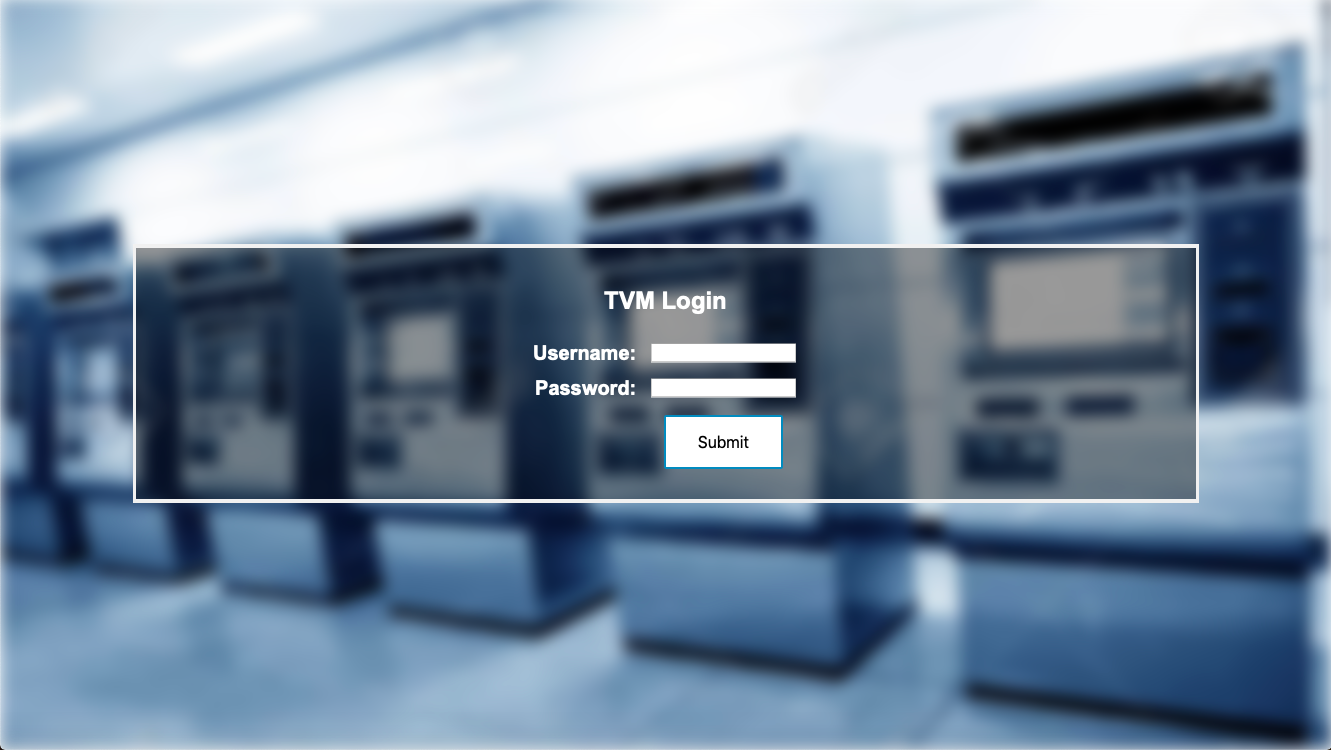
\includegraphics[width=18cm, height=12cm]{Implementation/TVM01.png}}
		\caption{\label{fig:tvm01}User Story: TVM-US-01}	
	\end{figure}
	
	\vspace{0.5cm}
	\textbf{DOM:} The implementation is done using the document object model of various HTMl elements. Elements are logically connected with each other and pass the values to verify the sequential alignment of all the elements and their corresponding functions.\\
	
	\vspace{0.5cm}
	\textbf{Data Structures: }The user is able to login into the system with a given username and password  Since we are not considering any database for the TVM application back end. The user will be able to login with a one user name and password only.\\
	
	\vspace{0.5cm}
	\textbf{Programming Platform: } HTML 5 and Javascript \\
	\textbf{User Interface:} Textual \\
	\textbf{Constraints covered:} Usability-G-01 \\
	
\end{flushleft}



%======================================================================
%				User Story: TVM-US-03
%======================================================================
\vspace{0.5cm}
\FloatBarrier
\subsection{Implementations - User Story: TVM-US-03}
As a Commuter, I want to be able to select ticket types (Rechargeable card or Non-rechargeable ticket), so that I can either reload Non-rechargeable card or buy a Rechargeable ticket.

\begin{flushleft}
	\textbf{Implementation}
	
	\vspace{0.5cm}
	\textbf{Instructions of Use}
	The TVM simulator for selecting ticket type will begin with the login and the displaying the ticket plans. Then the user is asked to select ticket types (Rechargeable card or Non-rechargeable ticket). If user inputs 1, Rechargable card is selected, if user selects 2 a Non-Rechargable ticket is selected.
	
	\begin{figure}[!htb]
		\fbox{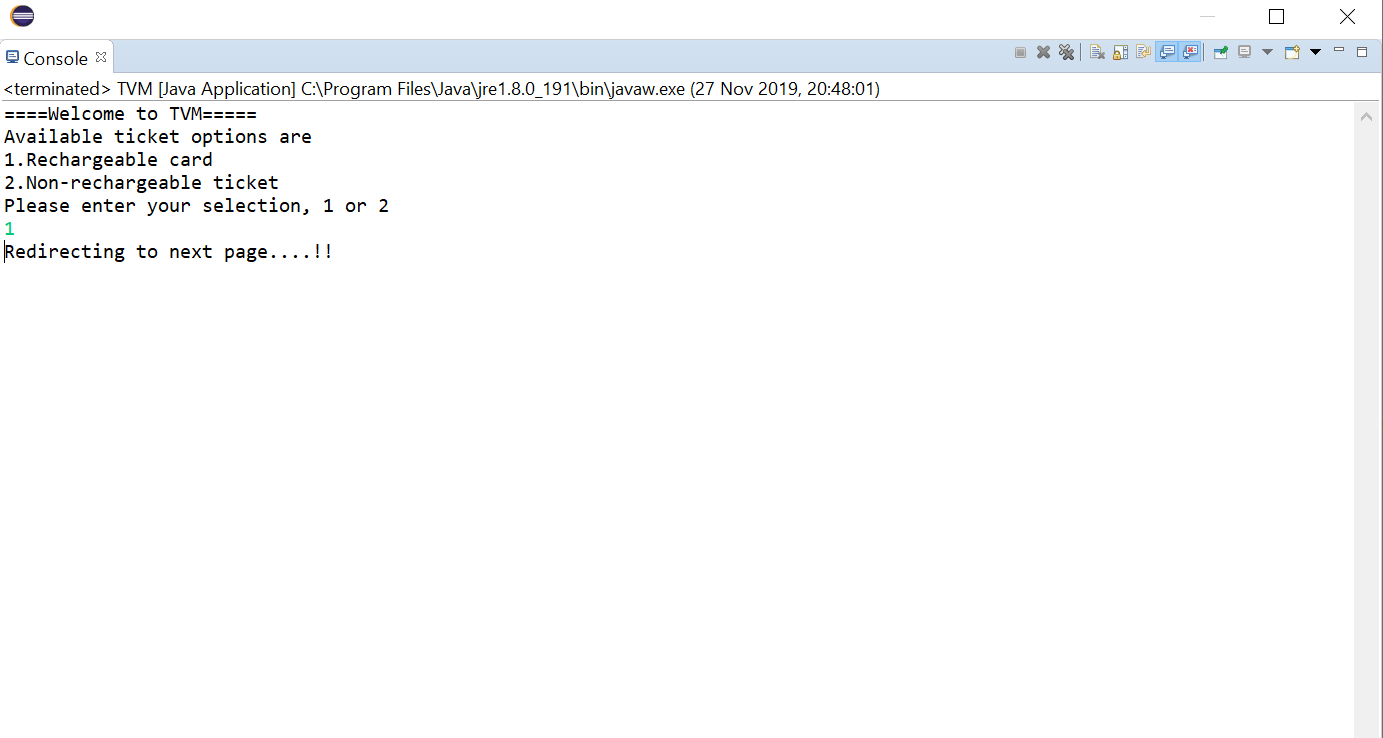
\includegraphics[width=18cm, height=8cm]{Implementation/TVM03_1.png}}
		\caption{\label{fig:tvm03_1}User Story: TVM-US-03}	
	\end{figure}

	\begin{figure}[!htb]
		\fbox{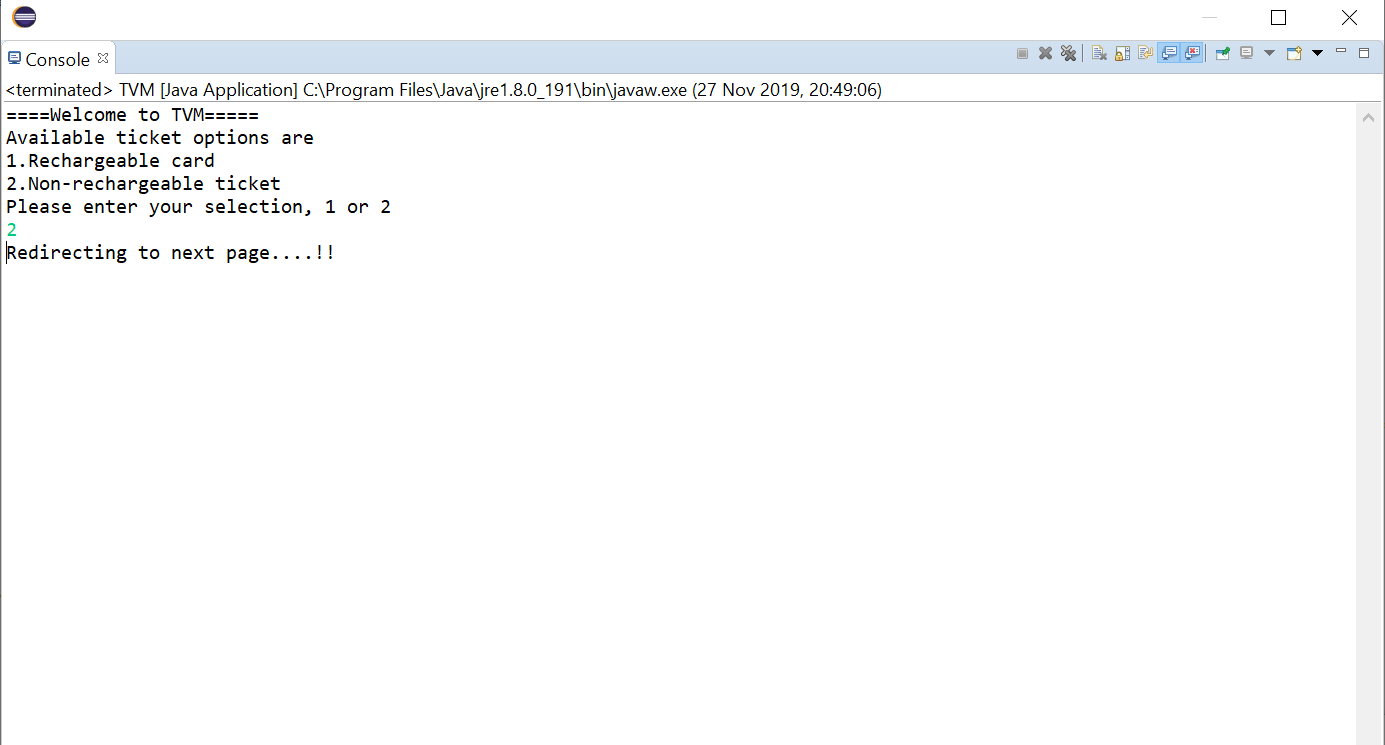
\includegraphics[width=18cm, height=8cm]{Implementation/TVM03_2.png}}
		\caption{\label{fig:tvm03_2}User Story: TVM-US-03}	
	\end{figure}
	
	\vspace{0.5cm}
	\textbf{DOM:} Since we are not considering any database for the TVM application back end. Basic data structures available in Java are taken. Ticket types are stored in an ArrayList.\\
	
	\vspace{0.5cm}
	\textbf{Data Structures: }The user is able to login into the system with a given username and password  Since we are not considering any database for the TVM application back end. The user will be able to login with a one user name and password only.\\
	
	\vspace{0.5cm}
	\textbf{Programming Platform: } Java Enterprise Edition \\
	\textbf{User Interface:} Textual \\
	\textbf{Constraints covered:} Performance-G-01 \\
	
	\vspace{0.5cm}
	\textbf{User Error Protection:} It will be made sure that user provides the right input in required format. \\
	\textbf{Maintainability: } Data structures selections are in such a way that any changes to the ticket types can be done. \\
	\textbf{Learnability: } New users will get to know that there are two types of tickets available i.e Rechargeable card or Non-rechargeable ticket
	
\end{flushleft}






%======================================================================
%				User Story: TVM-US-05
%======================================================================
\FloatBarrier
\vspace{0.5cm}
\subsection{Implementations - User Story: TVM-US-05}
As a Commuter, I want to be able to view ticket plans on selecting Non-rechargeable ticket with details and prices, so that I can decide what plan is suitable for me to buy.

This user story is implemented using Java with textual user interface. Since there is not a database so that system can read ticket information from a DB, a HashMap data structure is used to save the information about different ticket plans. Using console input/output user can communicate with the system.

\begin{flushleft}
	\textbf{Instruction of Use}
	This program is a Ticket Vending Machine simulator and displays ticket plans with details and fares to TVM user upon selecting Non-rechargeable ticket plans.
	When user selects the ticket type as "Non-rechargeable ticket" and selects to view ticket plans, this program displays the ticket plans and details to the user.
	First, the program description and the instruction are displayed to the user, then the list of ticket types is displayed to the user as shown in \ref{fig:tvm05} \\
	
	
	\begin{figure}[!htb]
		\fbox{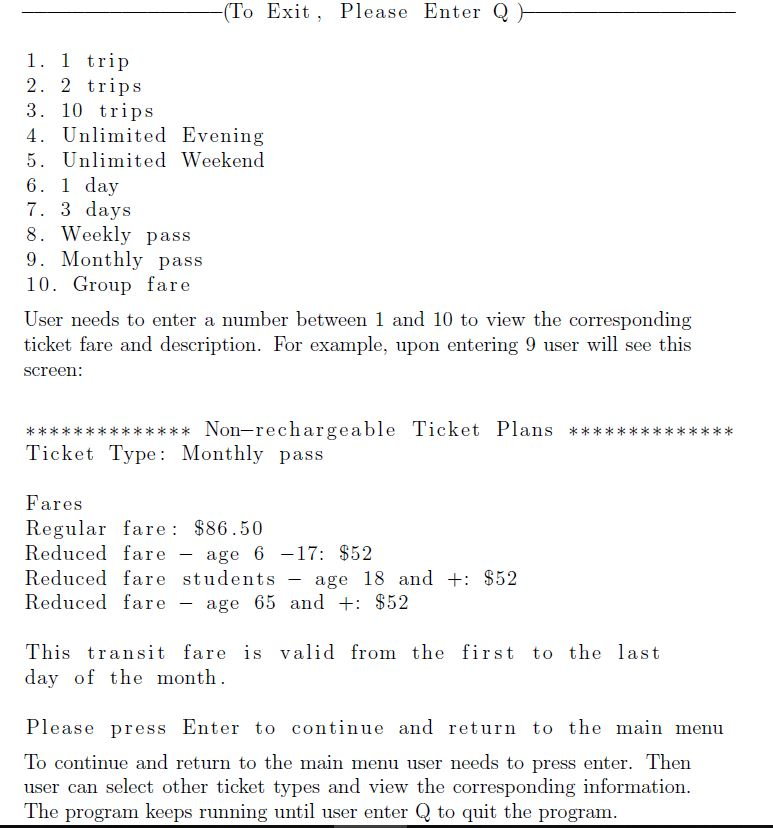
\includegraphics[width=18cm, height=19cm]{Implementation/TVM05.JPG}}
		\caption{\label{fig:tvm05}User Story: TVM-US-05}	
	\end{figure}
	
	\vspace{0.5cm}
	\textbf{Quality Attribute Constraints \cite{qualitykamthan}}
	
	\vspace{0.5cm}
	\textbf{Usability:} To increase user satisfaction usability quality attribute is considered as follow.\\
	
	\vspace{0.5cm}
	\textbf{Data Structures: }The user is able to login into the system with a given username and password  Since we are not considering any database for the TVM application back end. The user will be able to login with a one user name and password only.\\
	
	\vspace{0.5cm}
	\textbf{Programming Platform: } Java Enterprise Edition \\
	\textbf{User Interface:} Textual \\
	\textbf{Constraints covered:} Performance-G-01 \\
	
	\vspace{0.5cm}
	\textbf{User Error Protection:} The input is validated and if it is not a number an error message is displayed to user to correct the input. Also the input is verified to be in the correct range which is between 1 and 10, and if it is not in the valid range, an error message is displayed to the user as follow and user is asked to re-enter the input. \\
	\textbf{Usability:} To increase user satisfaction usability quality attribute is considered as follow.\\
	\textbf{Maintainability: } To increase maintainability, a HashMap data structure is dened which saves different ticket types and fares and details. With this implementation, if new plan needs to be added later, it can be added to the data structure with minimal modication. \\
	\textbf{Learnability: } At the beginning of the program, the type of program and its purpose is	displayed to the user and a user manual about how to use the system is 	displayed as well. \\
	\textbf{Operability: }To make the system operable, system keeps running until user enter "Q" to quite the program. Otherwise user can return to the main menu and view 	the detail for different ticket types. Also, to make the system understandable for the user, after showing the result of his/her request, the system freezes so that user can see the result. User asked to press enter to continue and return to the main menu. \\
	\textbf{Accessiblity: } In this project it is not possible to implement accessibility constraint which is using a screen reader as it needs hardware equipment which is not possible to prepare. \\
	
\end{flushleft}




%======================================================================
%				User Story: TVM-US-07
%======================================================================
\FloatBarrier
\vspace{0.5cm}
\subsection{Implementations - User Story: TVM-US-07}
As a commuter, I want to be able to make a payment using cash, So that I can purchase ticket and get confirmation receipt.

\begin{flushleft}
	\textbf{Implementation}
	The user story is implemented by using primitive types in which bill is displayed on the screen and user is asked to enter the amount for the cash. Then the user is requested to collect the balance and receipt. \\
	
	\textbf{Instructions of Use}
	The TVM simulator for payment by cash begins with displaying the bill. Then the user is asked to enter the amount for the payment. After the successful payment, the user is again asked to collect the balance and if he needs the transaction receipt. The receipt is printed based on the response of the user.
	
	\begin{figure}[!htb]
		\fbox{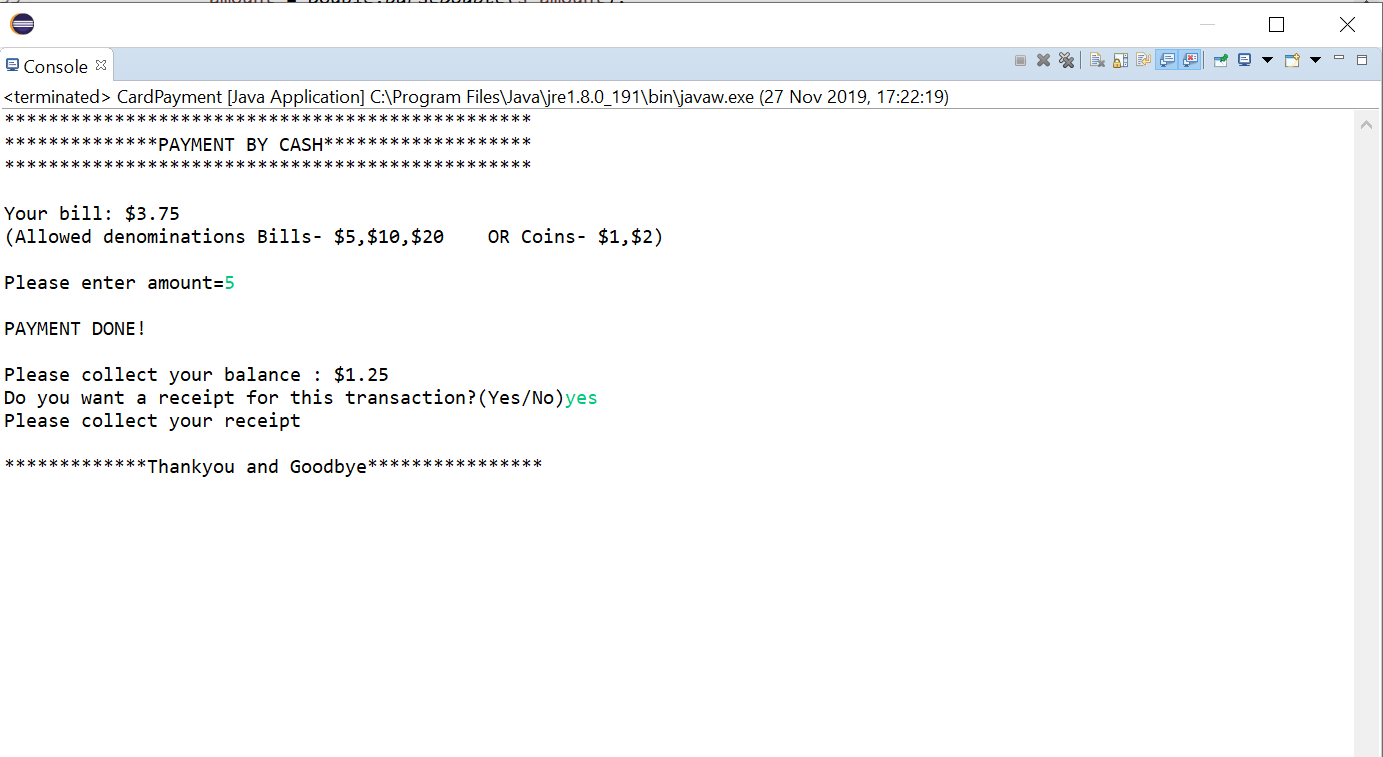
\includegraphics[width=18cm, height=10cm]{Implementation/TVM07.png}}
		\caption{\label{fig:tvm07}User Story: TVM-US-07}	
	\end{figure} 
	
	\vspace{0.5cm}
	\textbf{Programming Platform: } Java Enterprise Edition \\
	\textbf{User Interface:} Textual \\
	\textbf{Constraints covered:} Performance-G-01 \\
	
	\vspace{0.5cm}
	\textbf{User Error Protection:} It will be made sure that user provides the right input in required format. \\
	\textbf{Accessiblity: } In this project it is not possible to implement accessibility constraint which is using a screen reader as it needs hardware equipment which is not possible to prepare. \\
	
\end{flushleft}





%======================================================================
%				User Story: TVM-US-09
%======================================================================
\FloatBarrier
\vspace{0.5cm}
\subsection{Implementations - User Story: TVM-US-09}
As a commuter, I want to be able to cancel selected plan, So that I won't get charged and I can make changes later if I want in my purchase.

\begin{flushleft}
	\textbf{Implementation}
	The user story is implemented by using primitive types in which user selected plan is displayed to the user with options to "make a payment" or "cancel" the current transaction. Make a payment directs the user to the making a cash or card payment page while the cancel button directs user to homepage. \\ 
	
	\vspace{0.5cm}
	\textbf{Instructions of Use}
	\begin{itemize}
		\item Extract the Zip folder.
		\item Click on the PaymentPage.html file and open the file in browser.
		\item It will open a webpage for cancel functionality.
		\item The page will display two buttons – “cancel” and “make payment”.
		\item To make a payment for your selected plan click on “make payment” button and it will take you to the payment mode selection page
		\item To cancel a payment, click on “Cancel” button which will take you to the homepage of TVM.
	\end{itemize}
	
	\begin{figure}[!htb]
		\fbox{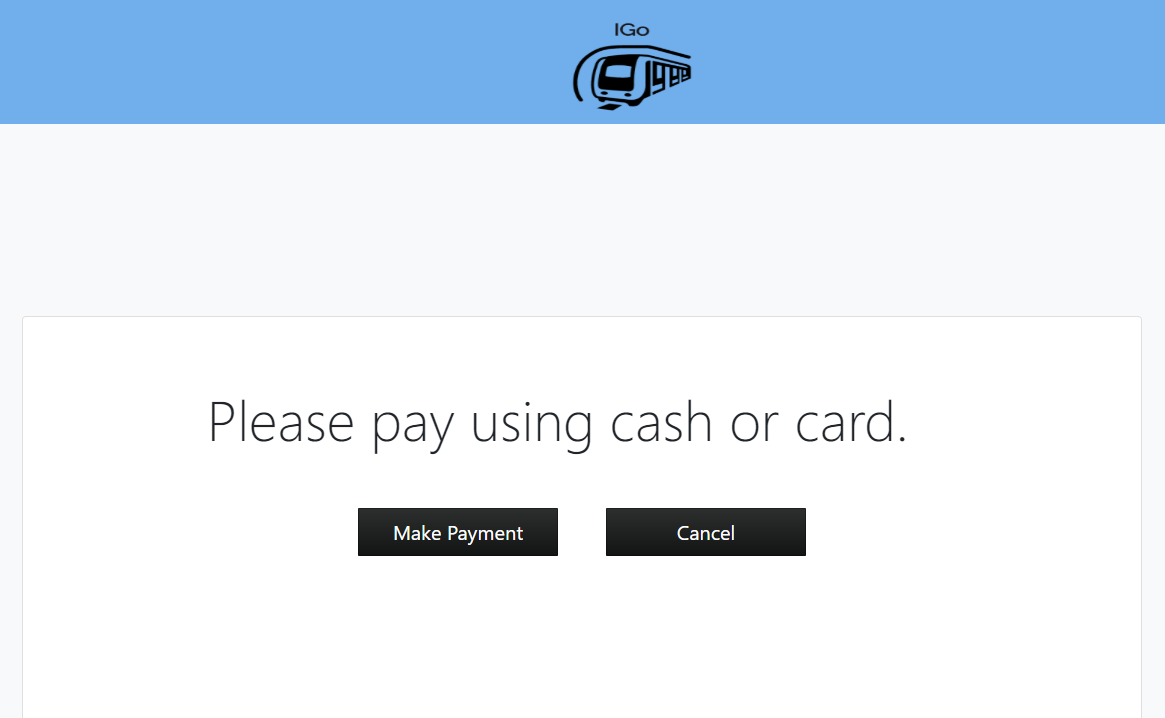
\includegraphics[width=18cm, height=10cm]{Implementation/TVM09.PNG}}
		\caption{\label{fig:tvm09}User Story: TVM-US-09}	
	\end{figure}
	
	\vspace{0.5cm}
	\textbf{Programming Platform: } HTML, CSS, Bootstrap \\
	\textbf{User Interface:} Textual, Graphical \\
	\textbf{Constraints covered:} Performance-G-01 \\
	
	
	\vspace{0.5cm}
	\textbf{Quality Attribute Constraints}
	
	\vspace{0.5cm}
	\textbf{User Error Protection:} It will be made sure that user provides the right input. At this screen the system has only 2 active buttons on the GUI that is either move to payment screen or cancel the transaction. No other input from user will be considered. \\
	\textbf{Maintainability: } The system does not depend on other modules for data and can easily me modified as per the future requirements. \\
	\textbf{Learnability: } User will be displayed only the necessary interaction components on the GUI. By hiding irrelevant details on payment selection screen makes it easier for user to navigate to the other steps. \\
	\textbf{Acessiblity: } In this project it is not possible to implement accessibility constraint which is using a screen reader. Also there will be a 3.5mm jack provided on the tvm for the visually impaired users which is also not possible to demonstrate here as it is hardware dependent. \\
	
\end{flushleft}


%=================================================================
%
%					APPENDIX PAGE
%
%==================================================================

\printbibliography[heading=subbibliography,title=References]

\printglossaries

\appendix
\addcontentsline{toc}{section}{Appendices}
\renewcommand{\thesection}{\Alph{section}}
\section{Appendix}
\subsection{Interviews}
Users are Interviewed and the results are accessable at: \href{https://github.com/m3hrn4z/SRS}{https://github.com/m3hrn4z/SRS}



\end{document}